\documentclass[11pt,a4paper]{article}
\usepackage[T2A]{fontenc}
\usepackage[utf8]{inputenc}
\usepackage[russian]{babel}
\usepackage{amsmath,amssymb}
\usepackage{graphicx}
\usepackage{booktabs}
\usepackage{multirow}
\usepackage{subcaption}
\usepackage{tikz}
\usepackage{xcolor}
\usepackage{listings}
\lstdefinestyle{py}{%
  language=Python,
  basicstyle=\ttfamily\scriptsize,
  keywordstyle=\color{blue!60!black}\bfseries,
  commentstyle=\color{gray!55!black}\itshape,
  stringstyle=\color{green!35!black},
  numbers=left, numberstyle=\tiny\color{gray!70}, numbersep=7pt,
  showstringspaces=false, breaklines=true, tabsize=4,
  columns=fullflexible, keepspaces=true,
  frame=single, framerule=0.3pt, rulecolor=\color{gray!45},
  backgroundcolor=\color{gray!5},
  captionpos=b, aboveskip=7pt, belowskip=4pt,
  % кириллица в телах листингов (pdflatex + T2A)
  extendedchars=true,
  literate=%
    {а}{{\cyra}}1 {б}{{\cyrb}}1 {в}{{\cyrv}}1 {г}{{\cyrg}}1 {д}{{\cyrd}}1 {е}{{\cyre}}1%
    {ё}{{\cyryo}}1 {ж}{{\cyrzh}}1 {з}{{\cyrz}}1 {и}{{\cyri}}1 {й}{{\cyrishrt}}1 {к}{{\cyrk}}1%
    {л}{{\cyrl}}1 {м}{{\cyrm}}1 {н}{{\cyrn}}1 {о}{{\cyro}}1 {п}{{\cyrp}}1 {р}{{\cyrr}}1%
    {с}{{\cyrs}}1 {т}{{\cyrt}}1 {у}{{\cyru}}1 {ф}{{\cyrf}}1 {х}{{\cyrh}}1 {ц}{{\cyrc}}1%
    {ч}{{\cyrch}}1 {ш}{{\cyrsh}}1 {щ}{{\cyrshch}}1 {ъ}{{\cyrhrdsn}}1 {ы}{{\cyrery}}1 {ь}{{\cyrsftsn}}1%
    {э}{{\cyrerev}}1 {ю}{{\cyryu}}1 {я}{{\cyrya}}1 {А}{{\CYRA}}1 {Б}{{\CYRB}}1 {В}{{\CYRV}}1%
    {Г}{{\CYRG}}1 {Д}{{\CYRD}}1 {Е}{{\CYRE}}1 {Ё}{{\CYRYO}}1 {Ж}{{\CYRZH}}1 {З}{{\CYRZ}}1%
    {И}{{\CYRI}}1 {Й}{{\CYRISHRT}}1 {К}{{\CYRK}}1 {Л}{{\CYRL}}1 {М}{{\CYRM}}1 {Н}{{\CYRN}}1%
    {О}{{\CYRO}}1 {П}{{\CYRP}}1 {Р}{{\CYRR}}1 {С}{{\CYRS}}1 {Т}{{\CYRT}}1 {У}{{\CYRU}}1%
    {Ф}{{\CYRF}}1 {Х}{{\CYRH}}1 {Ц}{{\CYRC}}1 {Ч}{{\CYRCH}}1 {Ш}{{\CYRSH}}1 {Щ}{{\CYRSHCH}}1%
    {Ъ}{{\CYRHRDSN}}1 {Ы}{{\CYRERY}}1 {Ь}{{\CYRSFTSN}}1 {Э}{{\CYREREV}}1 {Ю}{{\CYRYU}}1 {Я}{{\CYRYA}}1,
}
\usepackage[margin=2.3cm]{geometry}
\usepackage{caption}
\usepackage[hidelinks]{hyperref}
\usepackage[section]{placeins}
\usepackage{etoolbox}
% список источников — нумерованный раздел 4, а не безымянный
\patchcmd{\thebibliography}{\section*{\refname}}{\section{\refname}}{}{}
\addto\captionsrussian{\renewcommand{\refname}{Источники}}
\renewcommand{\topfraction}{0.9}
\renewcommand{\bottomfraction}{0.7}
\renewcommand{\textfraction}{0.08}
\renewcommand{\floatpagefraction}{0.75}
\setcounter{topnumber}{3}
\setcounter{bottomnumber}{2}
\setcounter{totalnumber}{5}
\graphicspath{{./}{figures/}{reference/screens/}}

\newcommand{\ao}{\vec a_\theta}
\newcommand{\af}{\vec a_\varphi}
\newcommand{\ar}{\vec a_r}
\newcommand{\Zl}{\overleftarrow{Z}}
\newcommand{\Zr}{\overrightarrow{Z}}
\newcommand{\Zb}{\overleftrightarrow{Z}}
\newcommand{\Yl}{\overleftarrow{Y}}
\newcommand{\Yb}{\overleftrightarrow{Y}}
\newcommand{\hn}{h_n^{(2)}}

\title{Ненормированные характеристики поля многослойных сферических тел:\\
расчёт методом тензорных функций Грина и верификация\\
полноволновым методом конечных элементов}
\author{}
\date{}

\begin{document}
\maketitle

\begin{abstract}
Приведены расчётные соотношения метода тензорных функций Грина (ТФГ) для
\emph{ненормированных} значений напряжённости поля многослойных сферических тел,
их реализация в библиотеке электродинамического анализа GreenTensor и верификация
полноволновым методом конечных элементов (Ansys HFSS). Рассмотрены обе задачи
возбуждения: дифракционная (плоская волна из дальней зоны) и антенная (источник на
поверхности структуры). Сопоставление выполнено по абсолютной величине --- в вольтах
на метр, без приведения к максимуму диаграммы --- для линейной поляризации
(вертикальной и горизонтальной) и круговой поляризации (по основной и
кросс-поляризации), всего по 30 диаграммам. Показано, что прямая запись антенного
возбуждения задаёт близкое к оптимальному сверхнаправленное возбуждение и потому
абсолютного уровня не задаёт; расчёт антенной задачи выполнен по соотношению
взаимности и согласуется с эталоном на том же уровне, что дифракционное.
Приведена таблица вычислительных затрат обоих методов.
\end{abstract}

\tableofcontents

\clearpage
\section{Постановка задачи дифракции на сферических телах}
\label{sec:diffraction}

Рассматривается радиально-слоистая сфера внешнего радиуса $a$, состоящая из $n$
концентрических слоёв с относительными электрическими радиусами границ
$k_0a = k_0a_n > k_0a_{n-1} > \dots > k_0a_1$; параметры слоёв описываются
значениями относительной диэлектрической $\varepsilon_i'$ и относительной магнитной
$\mu_i'$ проницаемости материала, внешняя среда --- вакуум. Конвенция времени
$e^{\,j\omega t}$, исходящая волна $\sim\hn(k_0r)$, $k_0 = 2\pi/\lambda_0$.

В дифракционной задаче на сферу падает электромагнитная волна: излучатель расположен
в дальней зоне ($r'\to\infty$) вдоль оси $z$, что моделирует плоский волновой фронт
вблизи дифракционного объекта. Напряжённость полного электрического поля $\mathbf{E}$
представляет собой сумму поля падающей волны $\mathbf{E}^i$ и поля рассеянной волны
$\mathbf{E}^s$; количественной мерой рассеивающих свойств объекта служит
$\mathbf{E}^s = \mathbf{E} - \mathbf{E}^i$. Геометрия задачи приведена на
рис.~\ref{fig:geom-diff}.

Угол $\theta$ отсчитывается от оси $+z$: $\theta = 0$ отвечает обратному рассеянию,
$\theta = 180^\circ$ --- рассеянию вперёд. Плоскость $\varphi = 0$ далее называется
E-плоскостью, плоскость $\varphi = \pi/2$ --- H-плоскостью.

\begin{figure}[ht]
  \centering
  \begin{tikzpicture}[scale=1.05,>=latex]
    \fill[gray!10] (0,0) circle (1.55);
    \draw[thick] (0,0) circle (1.55);
    \draw[dashed,gray!70] (0,0) circle (1.10);
    \draw[dashed,gray!70] (0,0) circle (0.62);
    \node[font=\tiny] at (0,0.25) {$\varepsilon_1',\mu_1'$};
    \node[font=\tiny] at (0,0.87) {$\varepsilon_i',\mu_i'$};
    \draw[->,gray] (0,0) -- (216:1.55) node[midway,below,font=\tiny]{$a$};
    \draw[->] (0,0) -- (0,2.45) node[right,font=\tiny]{$z$};
    \draw[->] (0,0) -- (2.15,0) node[below,font=\tiny]{$x$};
    \foreach \x in {-1.05,-0.45,0.15,0.75}{
      \draw[->,thick,blue!65!black] (\x,2.95) -- (\x,1.95);}
    \node[blue!65!black,font=\tiny,align=center] at (1.72,2.72) {$\vec E^{\,i}$\\$k_0$};
    \draw[->,thick,red!70!black] (0,0) -- (145:2.75)
      node[above left,font=\tiny,align=center]{$\vec E^{\,s}$\\$r\!\to\!\infty$};
    \draw[->,thin] (0,0.8) arc (90:145:0.8);
    \node[font=\tiny] at (114:1.05) {$\theta$};
    \node[font=\tiny,gray!60!black] at (0,-1.95) {$\theta=180^\circ$ --- рассеяние вперёд};
    \node[font=\tiny,gray!60!black] at (0.05,2.62) {$\theta=0$ --- обратное рассеяние};
  \end{tikzpicture}
  \caption{Геометрия задачи дифракции на радиально-слоистой сфере внешнего радиуса
  $a$: удалённый источник вдоль оси $z$ формирует плоский волновой фронт, точка
  наблюдения задана координатами $(r,\theta,\varphi)$}
  \label{fig:geom-diff}
\end{figure}

\subsection{Теория: ненормированные значения напряжённости поля}
\label{sec:theory-diff}

Базовый аппарат метода изложен в~\cite{denisov2016tensors}. Из него используются
без изменений: модель удалённого источника --- универсальная конфигурация на основе
суперпозиции вибраторов с амплитудным параметром $\alpha$ и фазовым сдвигом $\psi$;
характеристические части тензора Грина и их односторонние импедансы $\Zl_n$,
адмитансы $\Yl_n$ с рекурсией по слоям через функции $C_n$, $S_n$; двусторонние
величины $\Zb_n$, $\Yb_n$; амплитудные коэффициенты рассеяния
%
\begin{align}
  \label{eq:Mn}
  M_n &= \frac{j\Zl_n(a)\,j_n(k_0a) - j_n'(k_0a)}{j\Zb_n(a)\,\hn(k_0a)}, &
  N_n &= \frac{j\Yl_n(a)\,j_n(k_0a) - j_n'(k_0a)}{j\Yb_n(a)\,\hn(k_0a)};
\end{align}
%
угловые функции $\pi_n(\theta)$, $\tau_n(\theta)$; безразмерные компоненты поля для
линейной ($E_\theta$, $E_\varphi$) и круговой (по основной поляризации $E_{op}$ и
кросс-поляризации $E_{kp}$) поляризации. Число удерживаемых гармоник задаётся
критерием Уискомба $N_{\max} = \lceil x + 4x^{1/3} + 2\rceil$, $x = k_0a$~\cite{wiscombe1980}.

Поле падающей волны у объекта рассеяния определяется через элементарный
вибратор~\cite[ф-ла~3.18]{panchenko2013}:
%
\begin{equation}
  \label{eq:E0}
  E_0 = j\,\frac{I^e k_0 l Z_0}{4\pi}\cdot\frac{e^{-jk_0r'}}{r'},
  \qquad Z_0 = 376{,}730\ \text{Ом}.
\end{equation}
%
Для антенной задачи (раздел~\ref{sec:antenna}) облучателем служит элемент Гюйгенса
--- комбинированный источник со скрещёнными тангенциальными электрическим и
магнитным токами~\cite[ф-ла~3.14]{panchenko2013} с собственной кардиоидной
диаграммой $(1+\cos\theta)/2$ и амплитудой
%
\begin{equation}
  \label{eq:E0-huy}
  E_0^{(\text{Гюйг})} = \frac{I^{e}k_0lZ_0}{2\pi r}\,e^{-jk_0r}.
\end{equation}
%
По модулю \eqref{eq:E0-huy} вдвое больше \eqref{eq:E0}: знаменатель $2\pi$ вместо
$4\pi$.

Величины $E_\theta$, $E_\varphi$, $E_{op}$, $E_{kp}$ безразмерны: при переходе к
диаграмме $|F_\theta^s(\theta)| = |S_\parallel(\theta)|/(k_0a)$ множитель $E_0$
сокращается, и потому в теоретической записи он опускается. Ненормированная
напряжённость рассеянного поля в точке наблюдения на расстоянии $r$ получается
умножением на
%
\begin{equation}
  \label{eq:abs-lin}
  \boxed{\;
  \bigl|E_\theta^s(\theta,\varphi)\bigr| = \frac{E_0}{k_0r}\,\bigl|E_\theta\bigr|,
  \qquad
  \bigl|E_\varphi^s(\theta,\varphi)\bigr| = \frac{E_0}{k_0r}\,\bigl|E_\varphi\bigr|
  \quad [\text{В/м}],\;}
\end{equation}
%
где $E_0$ --- амплитуда падающей плоской волны у объекта (в расчётах настоящей
работы $E_0 = 1$~В/м), множитель $e^{-jk_0r}$ опущен как несущественный для модуля.
Для круговой поляризации амплитудный пакет содержит дополнительный множитель $1/2$,
поскольку величины $E_{op}$, $E_{kp}$ записаны как сумма и разность амплитуд
$S_\parallel$, $S_\perp$ и не нормированы на единичную амплитуду падающей волны
круговой поляризации:
%
\begin{equation}
  \label{eq:circR}
  \bigl|E_{op}^s\bigr| = \frac{E_0}{2k_0r}\,\bigl|E_{op}\bigr|,
\end{equation}
\begin{equation}
  \label{eq:circL}
  \bigl|E_{kp}^s\bigr| = \frac{E_0}{2k_0r}\,\bigl|E_{kp}\bigr| .
\end{equation}
%
Соответствие рукости: $E_{op}\leftrightarrow$~RHCP, $E_{kp}\leftrightarrow$~LHCP.

Пакет \eqref{eq:abs-lin} справедлив в дальней зоне. Продолжение того же ряда на
произвольное расстояние $r > a$ получается заменой асимптотики радиальных функций
на точные~\cite[ф-лы~4.45,~4.50]{bohren1983}; при $\rho = k_0r$
%
\begin{align}
  \label{eq:near-Eth}
  E_\theta &= A\cos\varphi\sum_{n=1}^{\infty}j^{\,n}\frac{2n+1}{n(n+1)}
    \left[j\,M_n\tau_n\frac{\bigl[\rho\hn(\rho)\bigr]'}{\rho} - N_n\pi_n\hn(\rho)\right],\\
  \label{eq:near-Eph}
  E_\varphi &= -A\sin\varphi\sum_{n=1}^{\infty}j^{\,n}\frac{2n+1}{n(n+1)}
    \left[j\,M_n\pi_n\frac{\bigl[\rho\hn(\rho)\bigr]'}{\rho} - N_n\tau_n\hn(\rho)\right],\\
  \label{eq:near-Er}
  E_r &= A\cos\varphi\sum_{n=1}^{\infty}j^{\,n}\frac{2n+1}{n(n+1)}\,
    j\,M_n\,n(n+1)\sin\theta\,\pi_n\frac{\hn(\rho)}{\rho},
\end{align}
%
где $A$ --- амплитуда источника соответствующего режима. При $k_0r\to\infty$
асимптотики $\hn\to j^{\,n+1}e^{-j\rho}/\rho$ и
$\bigl[\rho\hn\bigr]'/\rho\to j^{\,n}e^{-j\rho}/\rho$ переводят
\eqref{eq:near-Eth}--\eqref{eq:near-Eph} в \eqref{eq:abs-lin}: нормировка ближнего
поля наследуется из дальней зоны аналитически. Внутри тела ($r < a$) ряд исходящих
волновых функций расходится, что является свойством разложения; эти точки
маскируются.

Компоненты линейной поляризации умножаются на множитель
$(1-\sin^2\theta\cos^2\varphi)^{-1/2}$ --- обратную длину орта основной
поляризации:
%
\begin{equation}
  \label{eq:eco}
  \hat e_{\text{оп}} = \frac{\hat x - (\hat x\cdot\hat r)\,\hat r}
                            {\bigl|\hat x - (\hat x\cdot\hat r)\,\hat r\bigr|},
  \qquad
  \bigl|\hat x - (\hat x\cdot\hat r)\,\hat r\bigr| = \sqrt{1-\sin^2\theta\cos^2\varphi} .
\end{equation}
%
Суммы для $E_\theta$, $E_\varphi$ дают проекцию поля на ненормированный вектор в
числителе \eqref{eq:eco}; деление на его длину переводит результат в составляющую
вдоль единичного орта и абсолютного масштаба не затрагивает. В H-плоскости
($\varphi = 90^\circ$) множитель равен единице, в E-плоскости ($\varphi = 0$) ---
$1/|\cos\theta|$, и сокращает геометрический множитель $\cos\theta$, восстанавливая
$|S_\parallel(\theta)|$. В направлении $\theta = 90^\circ$, $\varphi = 0$ множитель
сингулярен, поэтому угловая сетка строится со смещением от особых точек.

Коэффициент $M_n$, получаемый из импеданса, отвечает электрической (TM) гармонике и
стоит при $\tau_n$ на орте $\ao$; коэффициент $N_n$, получаемый из адмиттанса, ---
магнитной (TE) гармонике и стоит при $\pi_n$~\cite{bhmie}.

\subsection{Реализация в библиотеке GreenTensor}
\label{sec:impl-diff}

Добавления раздела~\ref{sec:theory-diff} реализованы в библиотеке
электродинамического анализа GreenTensor (модуль \texttt{green\_tensor}); точным
матядром служит файл \texttt{01\_sphere.py}, импортируемым фасадом ---
\texttt{sphere\_core.py}.

\paragraph{Амплитуды источника.}
Листинг~\ref{lst:src} задаёт $E_0$ по \eqref{eq:E0} (метод \texttt{dipole\_e0}) и
амплитуду элемента Гюйгенса \eqref{eq:E0-huy} (метод \texttt{huygens\_e0}). Обе
величины возвращаются комплексными, с множителем $e^{-jk_0r}/r$ внутри; отношение
знаменателей $4\pi$ и $2\pi$ видно непосредственно, что и делает разницу в $6$~дБ
невозможной по недосмотру.

\begin{lstlisting}[style=py,caption={\texttt{green\_tensor/sphere\_core.py} ---
амплитуды источников \eqref{eq:E0} и \eqref{eq:E0-huy}},label={lst:src}]
Z0_FREE_SPACE = 376.730313668

@staticmethod
def dipole_e0(current, length, k0, r, z0=Z0_FREE_SPACE):
    return 1j * current * k0 * length * z0 / (4.0 * math.pi) * np.exp(-1j * k0 * r) / r

@staticmethod
def huygens_e0(current, length, k0, r, z0=Z0_FREE_SPACE):
    return current * k0 * length * z0 / (2.0 * math.pi * r) * np.exp(-1j * k0 * r)
\end{lstlisting}

\paragraph{Переход к ненормированным значениям.}
Листинг~\ref{lst:pack} реализует \eqref{eq:abs-lin}: безразмерные амплитуды $S_1$,
$S_2$ делятся на физическое волновое число $k$ и умножаются на $E_0$, что даёт
произведение $rE$ в вольтах; деление на расстояние $r$ переводит результат в В/м.
Отметим строку \texttt{k = self.k0 / radius}: внутри матядра
\texttt{self.k0} хранит безразмерный электрический радиус $k_0a$, и без этого
деления множитель $1/(k_0r)$ был бы вычислен при неверном волновом числе.
Возвращаемая величина $rE$ напрямую сопоставима с \texttt{rETheta}/\texttt{rEPhi}
полноволновых пакетов.

\begin{lstlisting}[style=py,caption={\texttt{sphere\_core.py::MieSphere.far\_field} ---
дифракционный амплитудный пакет \eqref{eq:abs-lin}},label={lst:pack}]
S1, S2 = self.amplitudes(theta)
k = self.k0 / float(radius)
out = {"rE_E": np.abs(S2) / k * e0,
       "rE_H": np.abs(S1) / k * e0}
if r is not None:
    out["E_E"] = out["rE_E"] / float(r)
    out["E_H"] = out["rE_H"] / float(r)
\end{lstlisting}

\paragraph{Круговая поляризация.}
Листинг~\ref{lst:circ} реализует \eqref{eq:circR}--\eqref{eq:circL}: переменная
\texttt{half} несёт множитель $E_0/(2k)$, где двойка --- выведенный, а не
подобранный коэффициент.

\begin{lstlisting}[style=py,caption={\texttt{sphere\_core.py::MieSphere.circular\_field}
--- абсолютные круговые компоненты \eqref{eq:circR}},label={lst:circ}]
k = self.k0 / float(radius)
half = abs(complex(e0)) / (2.0 * k)
out = {"rE_R": half * pat["E_op"], "rE_L": half * pat["E_kp"]}
if r is not None:
    out["E_R"] = out["rE_R"] / float(r)
    out["E_L"] = out["rE_L"] / float(r)
\end{lstlisting}

\paragraph{Точный радиальный ряд.}
Модуль \texttt{green\_tensor/nearfield.py} добавлен целиком.
Функция \texttt{\_hankel\_out} возвращает пару
$\bigl(\hn,\ [\rho\hn]'/\rho\bigr)$: вторая величина собирается как
\texttt{h / x + hp}, что и есть $\hn/\rho + \hn{}'$. Три строки сборки ---
дословная запись \eqref{eq:near-Eth}--\eqref{eq:near-Er}; фазовый вес \texttt{w}
содержит $j^{\,n}$, величины \texttt{a\_c}, \texttt{b\_c} --- коэффициенты $M_n$,
$N_n$ со снятым сопряжением. Точки $r < a$ маскируются значением \texttt{nan}.

\begin{lstlisting}[style=py,caption={\texttt{green\_tensor/nearfield.py} ---
\texttt{\_hankel\_out} (строки 1--3) и сборка точного радиального ряда
\eqref{eq:near-Eth}--\eqref{eq:near-Er}},label={lst:near}]
h  = jn + 1j * yn
hp = jnp + 1j * ynp
return h, h / x + hp

w   = (1j ** n) * (2 * n + 1) / (n * (n + 1))
Eth =  A * np.sum(w * (1j*a_c*taun*D - b_c*pin*h), axis=0) * cphi
Eph = -A * np.sum(w * (1j*a_c*pin*D - b_c*taun*h), axis=0) * sphi
Er  =  A * np.sum(w * (1j*a_c*n*(n+1)*np.sin(theta)*pin*h/rho_s), axis=0) * cphi
\end{lstlisting}

\paragraph{Множитель базисного орта.}
Листинг~\ref{lst:onkp} собирает $E_\theta$ и $E_\varphi$ по
формулам~\cite{denisov2016tensors}; величины \texttt{A} и \texttt{B} отвечают
комбинациям $(\tau_nM_n - \pi_nN_n)$ и $(\pi_nM_n - \tau_nN_n)$.
Переменная \texttt{norm} --- разобранный выше множитель
$(1-\sin^2\theta\cos^2\varphi)^{-1/2}$, то есть обратная длина орта \eqref{eq:eco};
абсолютный масштаб она не затрагивает.

\begin{lstlisting}[style=py,caption={\texttt{sphere\_core.py::MieSphere.pattern} ---
сборка линейной поляризации в базисе основной/кросс},label={lst:onkp}]
cphi, sphi = math.cos(self.phi), math.sin(self.phi)
cos_t = np.cos(theta)
A = tay * Mn_c - pii * Nn_c
B = pii * Mn_c - tay * Nn_c
s_teta = w * (-A * cos_t * cphi ** 2 - B * sphi ** 2)
s_phi  = w * (A * cphi * sphi - B * cos_t ** 2 * sphi * cphi)
E_teta = np.sum(s_teta, axis=0)
E_phi  = np.sum(s_phi,  axis=0)
norm   = (1 - (np.sin(theta) * cphi) ** 2) ** (-0.5)
E_teta = np.abs(norm * E_teta)
E_phi  = np.abs(norm * E_phi)
\end{lstlisting}

\paragraph{Расстановка угловых функций.}
Листинг~\ref{lst:ampl} воспроизводит рекуррентность для $\pi_n$, $\tau_n$ и сборку
амплитудных функций. Проверенная расстановка видна непосредственно: в $S_2$
(E-плоскость) коэффициент \texttt{Mn\_c} умножается на \texttt{taun}, в $S_1$
(H-плоскость) --- на \texttt{pin}.

\begin{lstlisting}[style=py,caption={\texttt{green\_tensor/\_angular.py::pi\_tau} и
\texttt{sphere\_core.py::MieSphere.amplitudes}},label={lst:ampl}]
pin[0] = 1.0
taun[0] = mu
if nmax >= 2:
    pin[1] = 3.0 * mu
    taun[1] = 2.0 * mu * pin[1] - 3.0 * pin[0]
for n in range(3, nmax + 1):
    i = n - 1
    pin[i]  = ((2*n - 1) / (n - 1)) * mu * pin[i-1] - (n / (n - 1)) * pin[i-2]
    taun[i] = n * mu * pin[i] - (n + 1) * pin[i-1]

w  = ((2 * n + 1) / (n * (n + 1)))[:, None]
S1 = np.sum(w * (Mn_c * pin + Nn_c * taun), axis=0)
S2 = np.sum(w * (Mn_c * taun + Nn_c * pin), axis=0)
\end{lstlisting}

\subsection{Верификационная модель в Ansys HFSS}
\label{sec:model-diff}

\paragraph{Рассматриваемые случаи.}
Эталонные модели построены для трёх тел при трёх значениях электрического радиуса
$k_0a$, охватывающих три качественно различных режима рассеяния: $k_0a = 0{,}5$ ---
рэлеевский ($k_0a \ll 1$), $k_0a = 2$ --- резонансный ($k_0a \sim 1$) и
$k_0a = 15$ --- квазиоптический ($k_0a \gg 1$). Частота моделирования во всех
случаях $f_0 = 10$~ГГц ($\lambda_0 = 29{,}98$~мм). Геометрия и материалы сведены в
таблицу~\ref{tab:geom}.

\begin{table}[ht]
  \centering
  \small
  \caption{Геометрия и материалы верификационных моделей. Для сферы с укрытием
  $k_0a$ относится к составному объекту, проводящее ядро имеет радиус $0{,}9a$}
  \label{tab:geom}
  \renewcommand{\arraystretch}{1.22}
  \begin{tabular}{@{}lccccl@{}}
    \toprule
    Тело & $k_0a$ & Ядро, мм & Внешний радиус, мм & $N_{\max}$ & Материалы (изнутри наружу) \\
    \midrule
    \multirow{3}{*}{Проводящая сфера}
      & $0{,}5$ & --- & $2{,}3857$  & 6  & PEC \\
      & $2$     & --- & $9{,}5426$  & 10 & PEC \\
      & $15$    & --- & $71{,}5695$ & 27 & PEC \\
    \midrule
    \multirow{3}{*}{Сфера с укрытием}
      & $0{,}5$ & $2{,}1471$  & $2{,}3857$  & 6  & PEC; ПТФЭ $\varepsilon = 2{,}1 - 4\cdot10^{-4}j$ \\
      & $2$     & $8{,}5883$  & $9{,}5426$  & 10 & PEC; ПТФЭ $\varepsilon = 2{,}1 - 4\cdot10^{-4}j$ \\
      & $15$    & $64{,}4126$ & $71{,}5695$ & 27 & PEC; ПТФЭ $\varepsilon = 2{,}1 - 4\cdot10^{-4}j$ \\
    \midrule
    Линза Люнеберга
      & $15$    & --- & $71{,}5702$ & 27 &
        $\varepsilon = 1{,}96 / 1{,}84 / 1{,}64 / 1{,}36 / 1{,}00$ \\
    \bottomrule
  \end{tabular}
\end{table}

Первое тело --- проводящая сфера без укрытия --- служит опорным случаем с
единственной границей. Второе --- проводящая сфера с диэлектрическим укрытием ---
вводит вторую границу и комплексную проницаемость; толщина укрытия $0{,}1a$.
Третье --- линза Люнеберга --- воспроизводит эталонный радиальный профиль
$\varepsilon(r) = 2 - (r/a)^2$~\cite{luneburg1944} ступенчатой аппроксимацией пятью
слоями при $r/a = 0{,}2$; $0{,}4$; $0{,}6$; $0{,}8$; $1{,}0$; внешний слой имеет
$\varepsilon = 1$, то есть геометрическая граница тела не является границей по
материалу --- дополнительная проверка того, что импедансная рекурсия корректно
обрабатывает вырожденный слой. Однородная шар-линза $\varepsilon = 4$, также
рассчитанная в этой серии, в настоящем документе не рассматривается.

Проводник моделируется как идеальный (PEC); в расчётной программе он задаётся слоем
с большой проницаемостью $\varepsilon = 10^{7}$. Достаточность этого значения
проверена сходимостью: при увеличении до $\varepsilon = 10^{11}$ коэффициент
обратного рассеяния $\sigma_r$ изменяется относительно не более чем на
$1{,}4\cdot10^{-3}$ ($k_0a = 0{,}5$), $2{,}1\cdot10^{-3}$ ($k_0a = 2$) и
$6{,}7\cdot10^{-3}$ ($k_0a = 15$).

\paragraph{Параметры источника.}
Возбуждение задано плоской волной единичной амплитуды $E_0 = 1$~В/м с поляризацией
вдоль оси $x$, распространяющейся вдоль $-z$. Ненормированный уровень поля,
рассчитываемый по \eqref{eq:abs-lin}, тем самым определён однозначно и одинаков для
обеих методик. Расстояние наблюдения для всех абсолютных величин
$r = 10$~м ($k_0r \approx 2{,}1\cdot10^{3}$), что заведомо соответствует дальней
зоне для наибольшего из размеров.

\paragraph{Постановка эталонного расчёта.}
Эталон получен полноволновым методом конечных элементов (Ansys HFSS 2024\,R2,
решение типа Driven Modal, базис первого порядка, $\Delta S = 0{,}02$, до 12
адаптивных проходов). Тело помещено в вакуумную область с граничным условием
Radiation (для $k_0a = 15$ --- PML), зазор до границы не менее $\lambda_0/4$.
Дальнее поле снято на бесконечной сфере (Infinite Sphere) в диапазоне
$\theta = 0\ldots360^\circ$ с шагом $1^\circ$ в срезах $\varphi = 0$ и
$\varphi = \pi/2$; экспортируются величины $rE$~[В], пересчитываемые в напряжённость
поля как $|E| = rE/r$. Круговая поляризация снята штатными величинами
\texttt{rELHCP}, \texttt{rERHCP} на той же сфере.

Модели в окне трёхмерного моделирования Ansys HFSS приведены на
рис.~\ref{fig:models-diff}. Сечение через центр линзы выявляет концентрическую
слоистую структуру, аппроксимирующую радиальный профиль проницаемости.

\begin{figure}[ht]
  \centering
  \begin{subfigure}[b]{0.325\textwidth}
    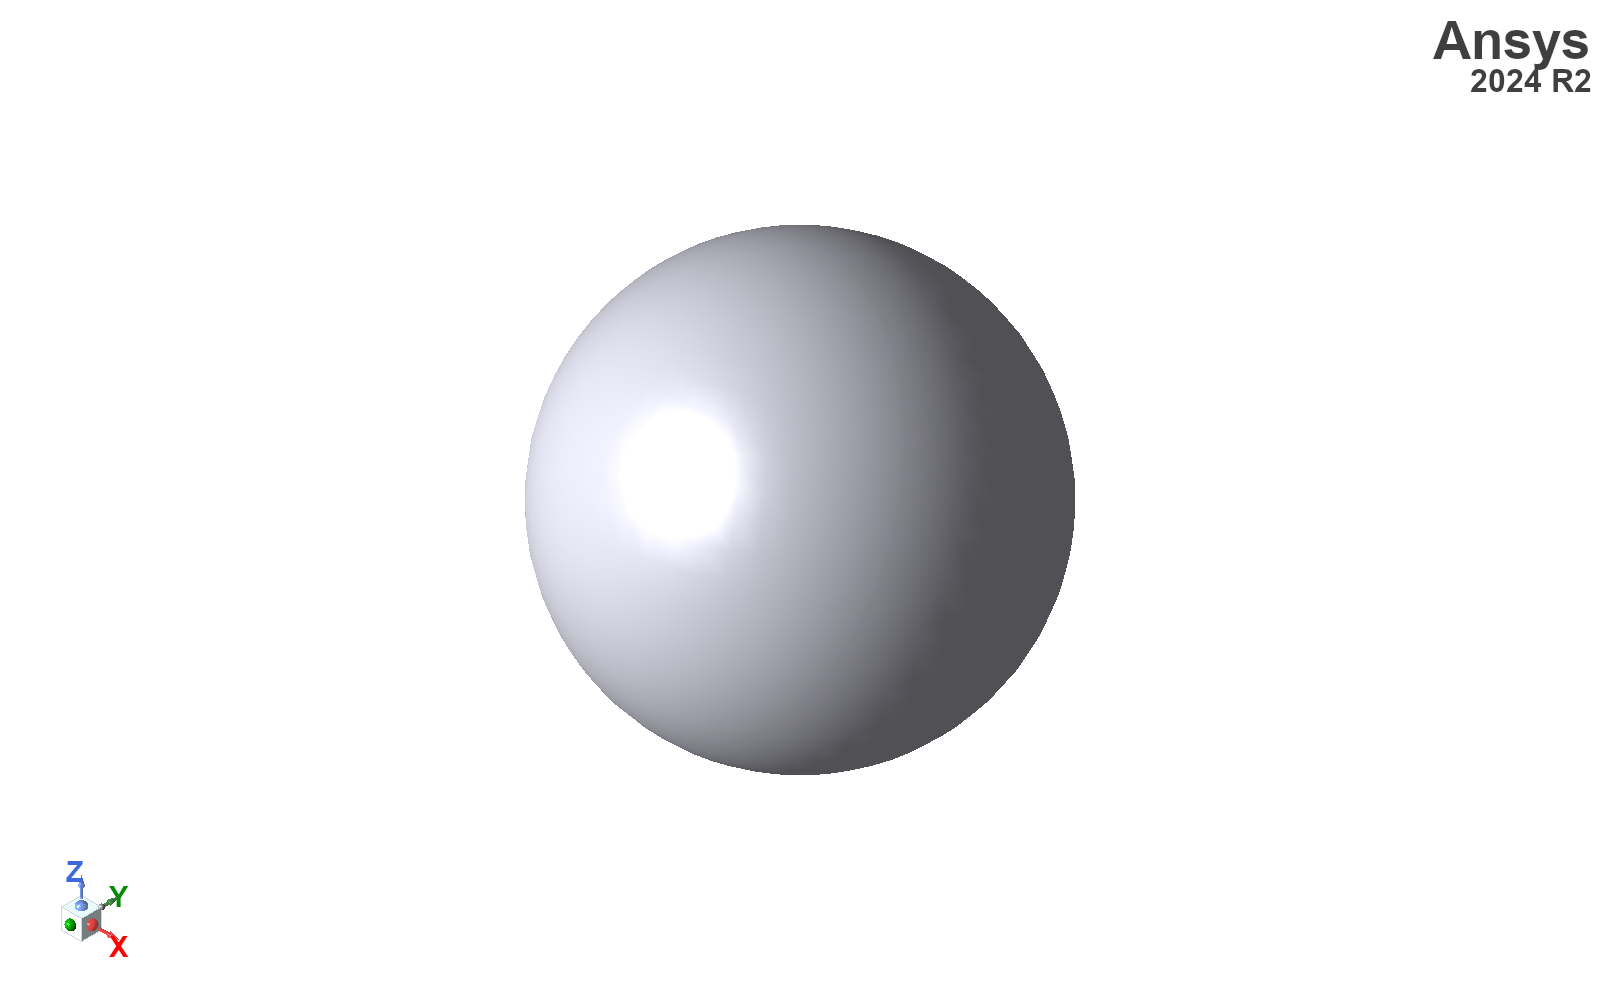
\includegraphics[width=\textwidth]{pec_k15_model_iso}
    \caption{проводящая сфера}
  \end{subfigure}\hfill
  \begin{subfigure}[b]{0.325\textwidth}
    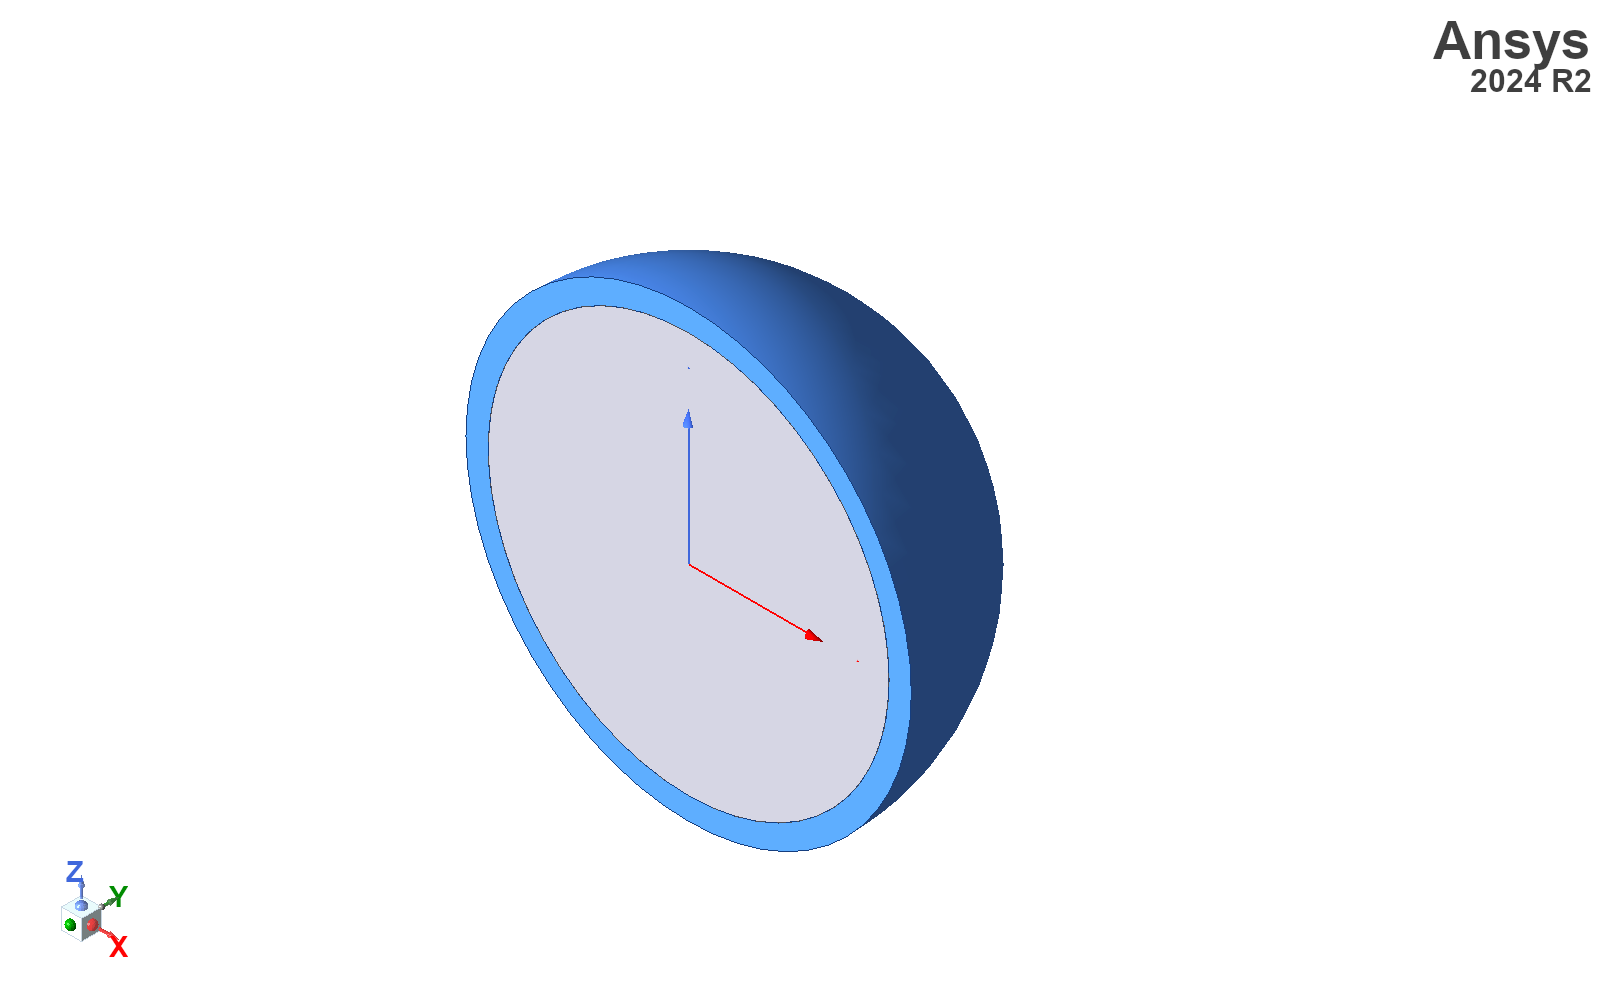
\includegraphics[width=\textwidth]{radome_k15_cutaway}
    \caption{сфера с укрытием, разрез}
  \end{subfigure}\hfill
  \begin{subfigure}[b]{0.325\textwidth}
    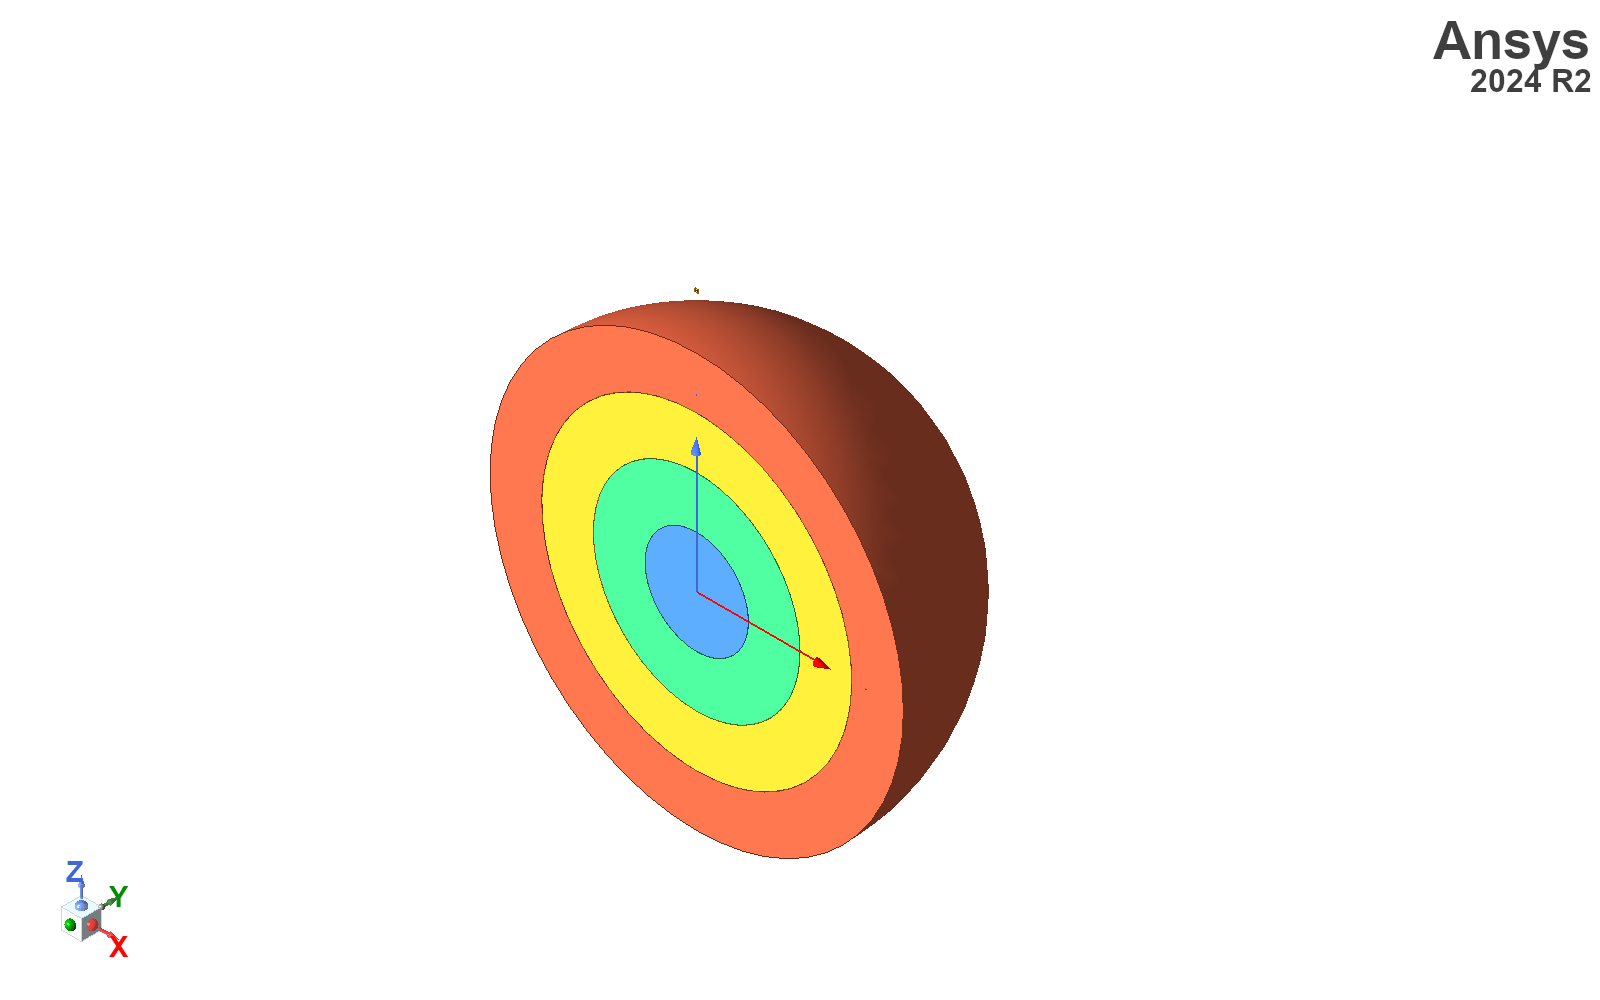
\includegraphics[width=\textwidth]{luneburg_k15_lens_cutaway_isometric}
    \caption{линза Люнеберга, разрез}
  \end{subfigure}
  \caption{Эталонные модели в окне трёхмерного моделирования Ansys HFSS при
  $k_0a = 15$: проводящая сфера, проводящая сфера с диэлектрическим укрытием
  (разрез выявляет слой ПТФЭ на проводящем ядре) и пятислойная линза
  Люнеберга (разрез выявляет концентрические слои)}
  \label{fig:models-diff}
\end{figure}

\subsection{Результаты верификации}
\label{sec:results-diff}

Для каждой конфигурации приведён набор из четырёх круговых диаграмм. Верхний ряд ---
линейная поляризация: слева вертикальная (E-плоскость, $\varphi = 0$), справа
горизонтальная (H-плоскость, $\varphi = 90^\circ$). Нижний ряд --- круговая
поляризация: слева основная ($E_{op}$), справа кросс-поляризация ($E_{kp}$). На
каждой диаграмме сопоставлена одна пара кривых --- расчёт методом ТФГ и
соответствующая ей величина полноволнового эталона. Ориентация всех диаграмм
одинакова: $\theta = 0$ (обратное рассеяние) вверху, отсчёт по часовой стрелке,
$\theta = 180^\circ$ (рассеяние вперёд) внизу. Радиальная шкала --- $20\lg|E|$ при
$|E|$ в В/м, единая для всех четырёх диаграмм набора, динамический диапазон 45~дБ.
Медиана расхождения вычислена по лепесткам выше $1\,\%$ от максимума.

\subsubsection{Проводящая сфера}
\label{sec:res-pec}


\paragraph{Вывод.}
Три набора (рис.~\ref{fig:pol-pec-05}--\ref{fig:pol-pec-15}) прослеживают
перестройку картины рассеяния с ростом электрического радиуса --- основного
параметра задачи.

При $k_0a = 0{,}5$ (рэлеевский режим) диаграмма вертикальной поляризации имеет вид
деформированной восьмёрки с максимумом в направлении обратного рассеяния:
рассеяние вперёд на $7{,}26$~дБ слабее обратного, что отвечает противофазному
сложению электрического и магнитного дипольных вкладов идеально проводящей сферы.
Диаграмма горизонтальной поляризации в этом режиме практически изотропна ---
угловая зависимость $\pi_n$ при $n = 1$ постоянна. Уровень поля составляет
$8{,}7\cdot10^{-5}$~В/м при падающей волне $1$~В/м, то есть на $81$~дБ ниже;
согласие по абсолютной величине: $-0{,}29$~дБ по максимуму вертикальной
поляризации, медиана $0{,}31$~дБ. Наибольшее расхождение набора приходится на
основную поляризацию круговой волны ($1{,}00$~дБ) --- эта величина по
$E_{op}$ есть разность $(\tau_n - \pi_n)$, и в рэлеевском пределе, где обе
угловые функции близки, она собирается как малая разность близких чисел.

При $k_0a = 2$ (резонансный режим) картина переворачивается: максимум переходит в
направление $\theta = 180^\circ$, рассеяние вперёд превышает обратное на
$7{,}11$~дБ. Появляется боковая структура, но лепестки ещё не разделены ---
диаграмма всюду выше $-20$~дБ от максимума. Согласие в этом режиме наиболее тесное по
всей серии: $+0{,}02$~дБ по максимуму, медиана $0{,}10$~дБ.

При $k_0a = 15$ (квазиоптический режим) диаграмма приобретает характерную
лепестковую структуру: узкий главный лепесток вперёд шириной $14{,}0^\circ$ по
уровню $-3$~дБ, рассеяние вперёд на $24{,}02$~дБ выше обратного, выше $-20$~дБ
остаются лишь 47 угловых узлов из 360. Это соответствует известному выводу о том,
что с ростом $k_0a$ рассеянное поле концентрируется в направлении распространения
падающей волны~\cite{denisov2016tensors}. Согласие $+0{,}23$~дБ по максимуму при
медиане $0{,}49$~дБ; остаточное расхождение сосредоточено в глубоких минимумах
между лепестками, где уровень мал и результат сеточного метода зависит от
дискретизации.

Во всех трёх наборах кросс-поляризационная компонента линейной задачи
($E_\varphi$ в главных плоскостях) даёт у метода ТФГ тождественный нуль, тогда как полноволновой расчёт
показывает $1{,}2\cdot10^{-6}$; $2{,}9\cdot10^{-5}$ и $1{,}5\cdot10^{-4}$~В/м ---
на $37{,}6$; $31{,}4$ и $51{,}1$~дБ ниже основной составляющей, то есть на уровне
численного шума сетки.

\begin{figure}[ht]
  \centering
  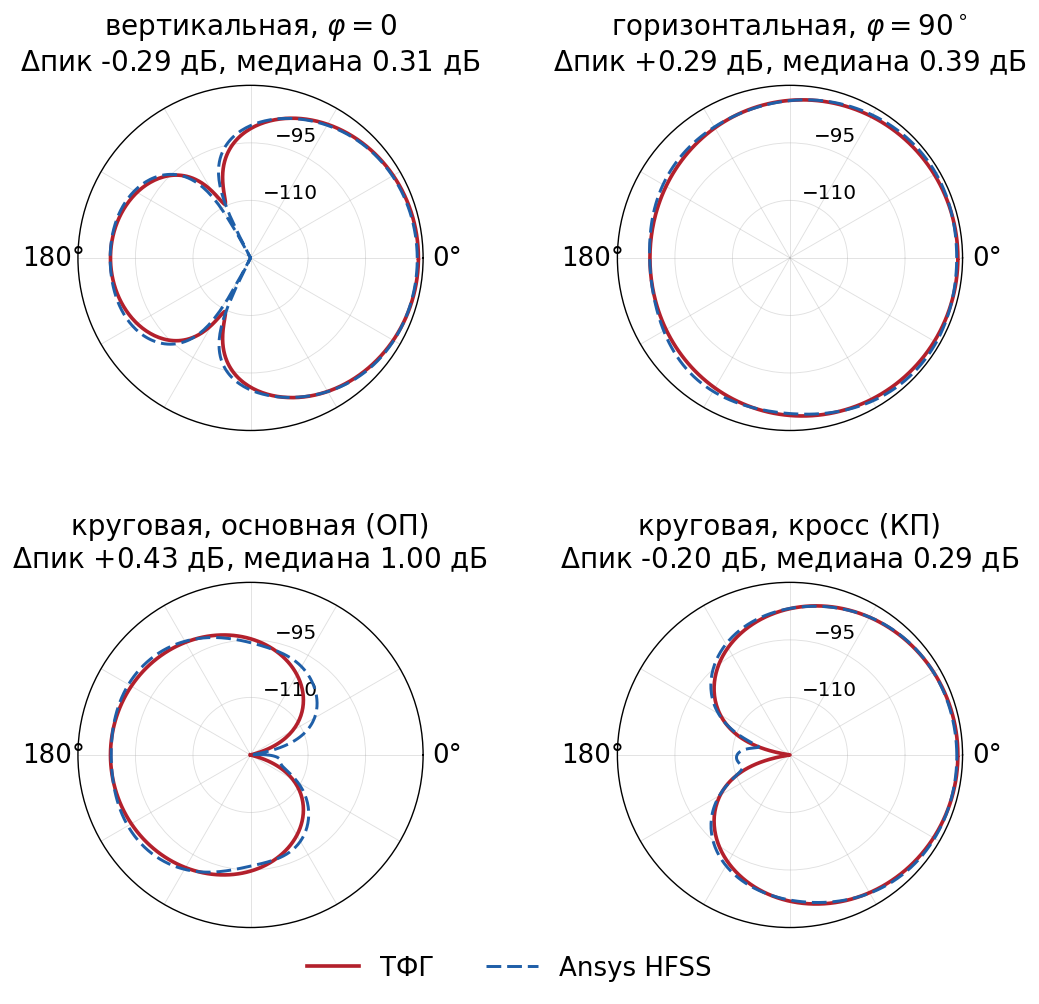
\includegraphics[width=0.98\textwidth]{pol_pec_k0p5_diffraction}
  \caption{Проводящая сфера, $k_0a = 0{,}5$: ненормированные диаграммы рассеяния
  метода ТФГ и полноволнового эталона}
  \label{fig:pol-pec-05}
\end{figure}

\begin{figure}[ht]
  \centering
  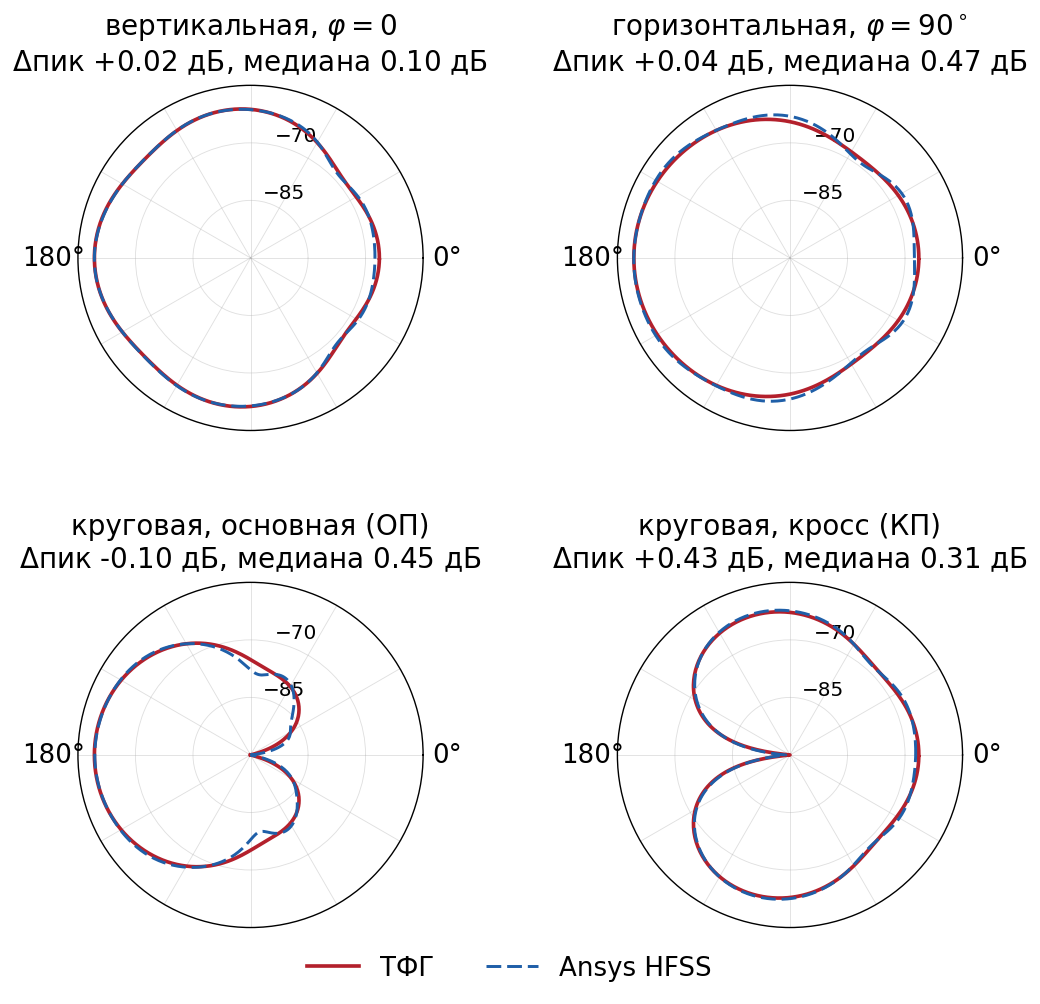
\includegraphics[width=0.98\textwidth]{pol_pec_k2_diffraction}
  \caption{Проводящая сфера, $k_0a = 2$: ненормированные диаграммы рассеяния
  метода ТФГ и полноволнового эталона}
  \label{fig:pol-pec-2}
\end{figure}

\begin{figure}[ht]
  \centering
  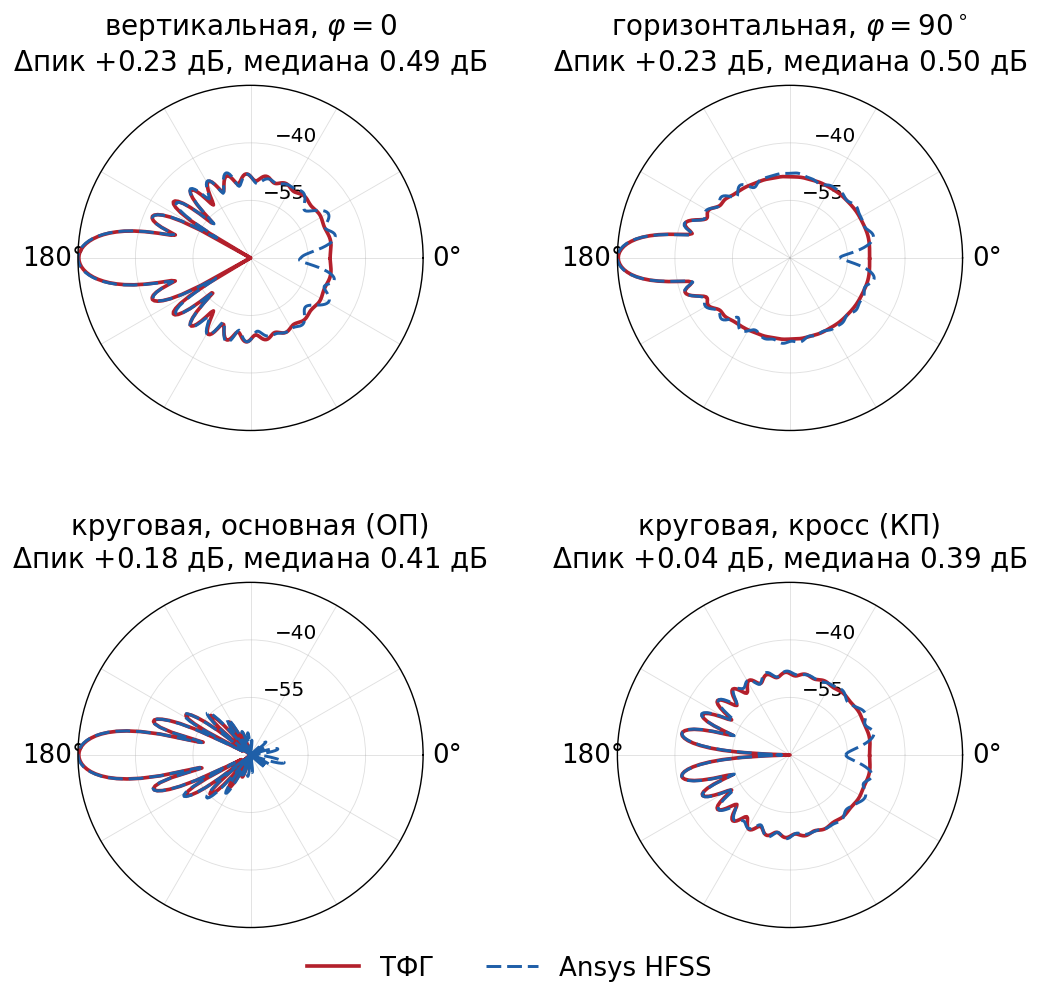
\includegraphics[width=0.98\textwidth]{pol_pec_k15_diffraction}
  \caption{Проводящая сфера, $k_0a = 15$: ненормированные диаграммы рассеяния
  метода ТФГ и полноволнового эталона}
  \label{fig:pol-pec-15}
\end{figure}

\FloatBarrier

\subsubsection{Сфера с диэлектрическим укрытием}
\label{sec:res-radome}


\paragraph{Вывод.}
Введение второй границы --- слоя ПТФЭ толщиной $0{,}1a$ на проводящем ядре ---
качественно картину не меняет: сохраняются и рэлеевский вид при $k_0a = 0{,}5$
(рис.~\ref{fig:pol-rad-05}), и переход к рассеянию вперёд при $k_0a = 2$
(рис.~\ref{fig:pol-rad-2}), и лепестковая структура при $k_0a = 15$
(рис.~\ref{fig:pol-rad-15}). Количественные различия с непокрытой сферой при этом
вполне определённые и воспроизводятся обеими методиками.

При $k_0a = 0{,}5$ укрытие ослабляет обратное рассеяние: отношение вперёд/назад
меняется с $-7{,}26$ на $-5{,}98$~дБ, а абсолютный уровень падает с
$8{,}7\cdot10^{-5}$ до $7{,}2\cdot10^{-5}$~В/м. При $k_0a = 2$ укрытие, напротив,
усиливает направленность вперёд --- отношение растёт с $+7{,}11$ до $+10{,}50$~дБ.
При $k_0a = 15$ главный лепесток сужается с $14{,}0^\circ$ до $12{,}0^\circ$
(увеличенный эффективный размер составного объекта), а обратное рассеяние
возрастает на $4{,}61$~дБ относительно непокрытой сферы --- вклад отражения от
внешней границы диэлектрика, складывающегося с отражением от ядра.

Согласие по абсолютной величине выдерживается на том же уровне, что и для
непокрытой сферы, и в резонансном режиме даже несколько лучше: расхождение
максимумов $-0{,}36$; $+0{,}05$; $+0{,}26$~дБ при медианах $0{,}25$; $0{,}14$;
$0{,}45$~дБ для трёх размеров соответственно. Наибольшее расхождение набора ---
$0{,}81$~дБ по основной поляризации круговой волны при $k_0a = 15$. Отметим, что
комплексная проницаемость укрытия ($\operatorname{tg}\delta \approx 1{,}9\cdot10^{-4}$)
и вторая граница не приводят к систематическому смещению уровня: знак расхождения
максимумов меняется от случая к случаю, что характерно для случайной погрешности
дискретизации, а не для ошибки нормировки.

\begin{figure}[ht]
  \centering
  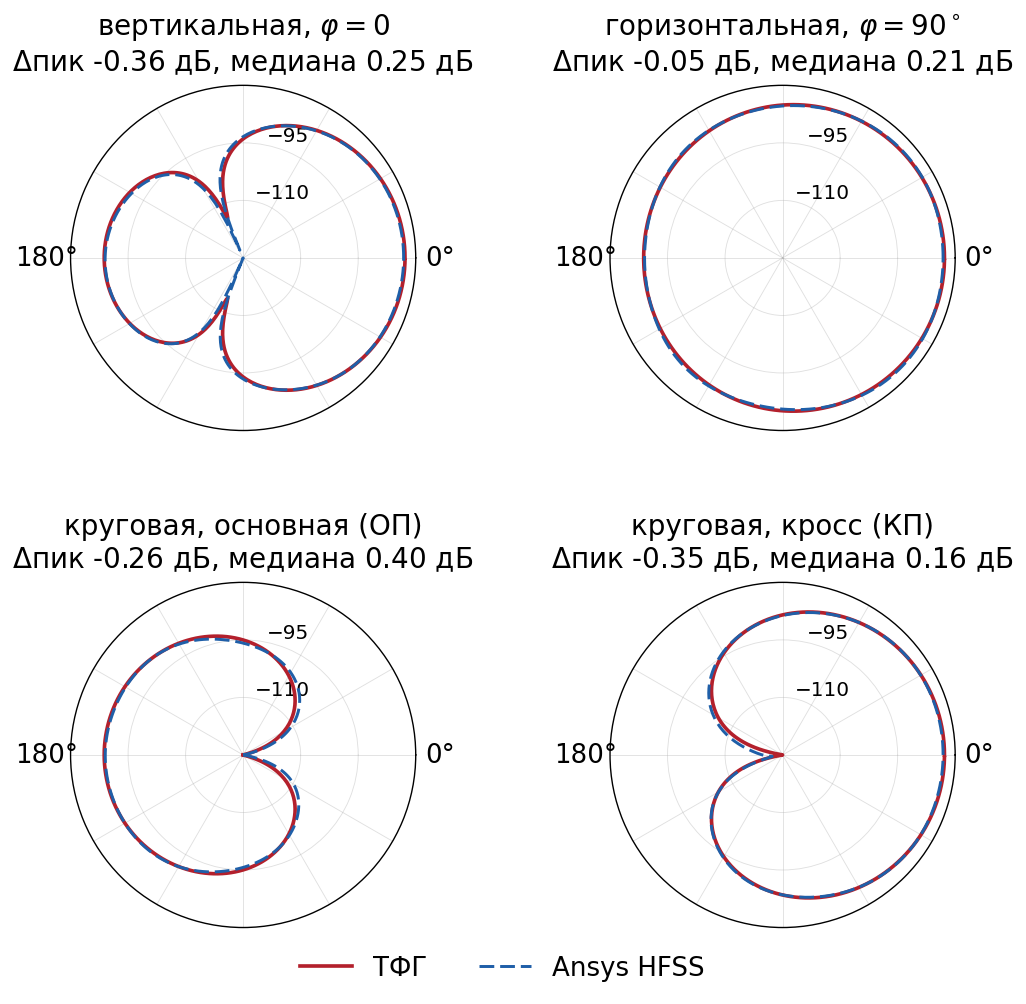
\includegraphics[width=0.98\textwidth]{pol_radome_k0p5_diffraction}
  \caption{Сфера с укрытием, $k_0a = 0{,}5$: ненормированные диаграммы рассеяния
  метода ТФГ и полноволнового эталона}
  \label{fig:pol-rad-05}
\end{figure}

\begin{figure}[ht]
  \centering
  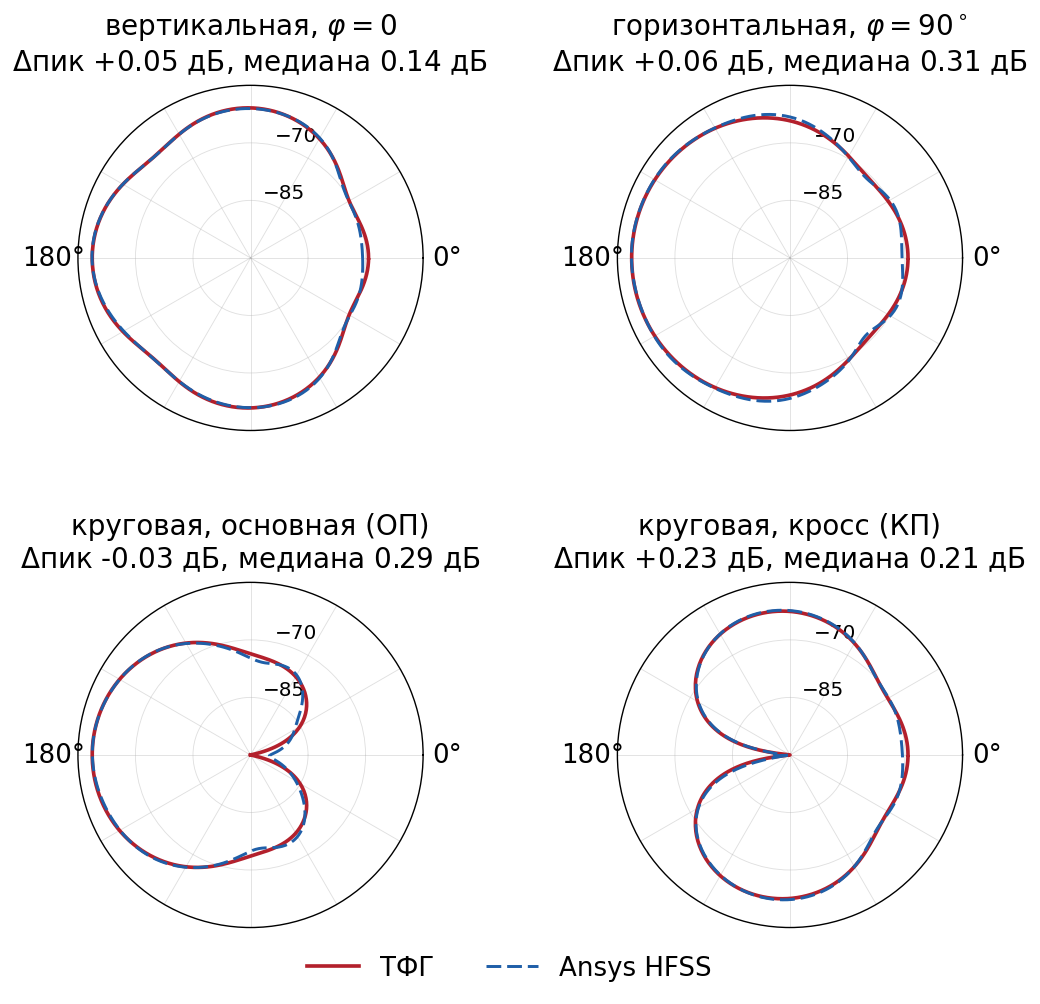
\includegraphics[width=0.98\textwidth]{pol_radome_k2_diffraction}
  \caption{Сфера с укрытием, $k_0a = 2$: ненормированные диаграммы рассеяния
  метода ТФГ и полноволнового эталона}
  \label{fig:pol-rad-2}
\end{figure}

\begin{figure}[ht]
  \centering
  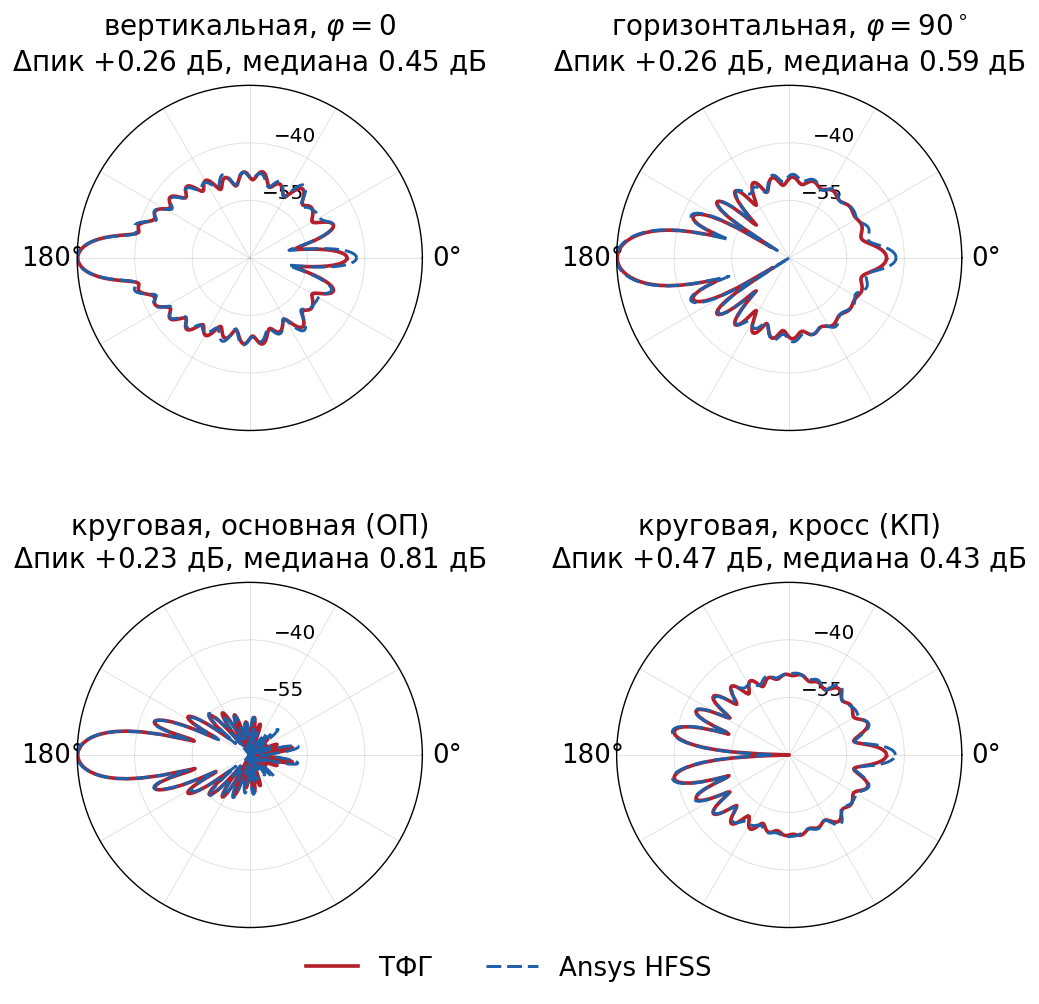
\includegraphics[width=0.98\textwidth]{pol_radome_k15_diffraction}
  \caption{Сфера с укрытием, $k_0a = 15$: ненормированные диаграммы рассеяния
  метода ТФГ и полноволнового эталона}
  \label{fig:pol-rad-15}
\end{figure}

\FloatBarrier

\subsubsection{Линза Люнеберга}
\label{sec:res-lun}


\paragraph{Вывод.}
Линза Люнеберга (рис.~\ref{fig:pol-lun}) проверяет метод там, где результат целиком
определяется импедансной рекурсией по слоям: у первых двух тел рассеяние формируется
одной-двумя границами, здесь --- пятью, причём внешняя из них вырождена
($\varepsilon = 1$).

Диаграмма сохраняет квазиоптический вид с максимумом вперёд ($+23{,}75$~дБ
относительно обратного, ширина главного лепестка $14{,}0^\circ$), но лепестковая
структура выражена сильнее, чем у проводящей сферы того же электрического
радиуса: выше $-20$~дБ остаются 113 угловых узлов против 47. Расхождение
максимумов $+0{,}25$~дБ, медиана $0{,}63$~дБ в E-плоскости и $1{,}13$~дБ в
H-плоскости --- несколько выше, чем у однородных тел, что отвечает пятикратному
увеличению числа границ в сеточной модели.

Отдельного комментария требует кросс-поляризация круговой волны: расхождение
максимума $+4{,}33$~дБ при медиане $1{,}81$~дБ --- худший показатель всей
дифракционной серии. Причина в том, что у этого тела величина $E_{kp}$ по
$E_{kp}$ собирается как разность $(M_n - N_n)$ и оказывается на $23{,}8$~дБ
ниже основной поляризации ($2{,}4\cdot10^{-3}$ против $3{,}7\cdot10^{-2}$~В/м).
Абсолютная величина расхождения при этом составляет $1{,}5\cdot10^{-3}$~В/м, то
есть менее $4\,\%$ от уровня основной поляризации; в остальных диаграммах набора
эта величина не проявляется.

\begin{figure}[ht]
  \centering
  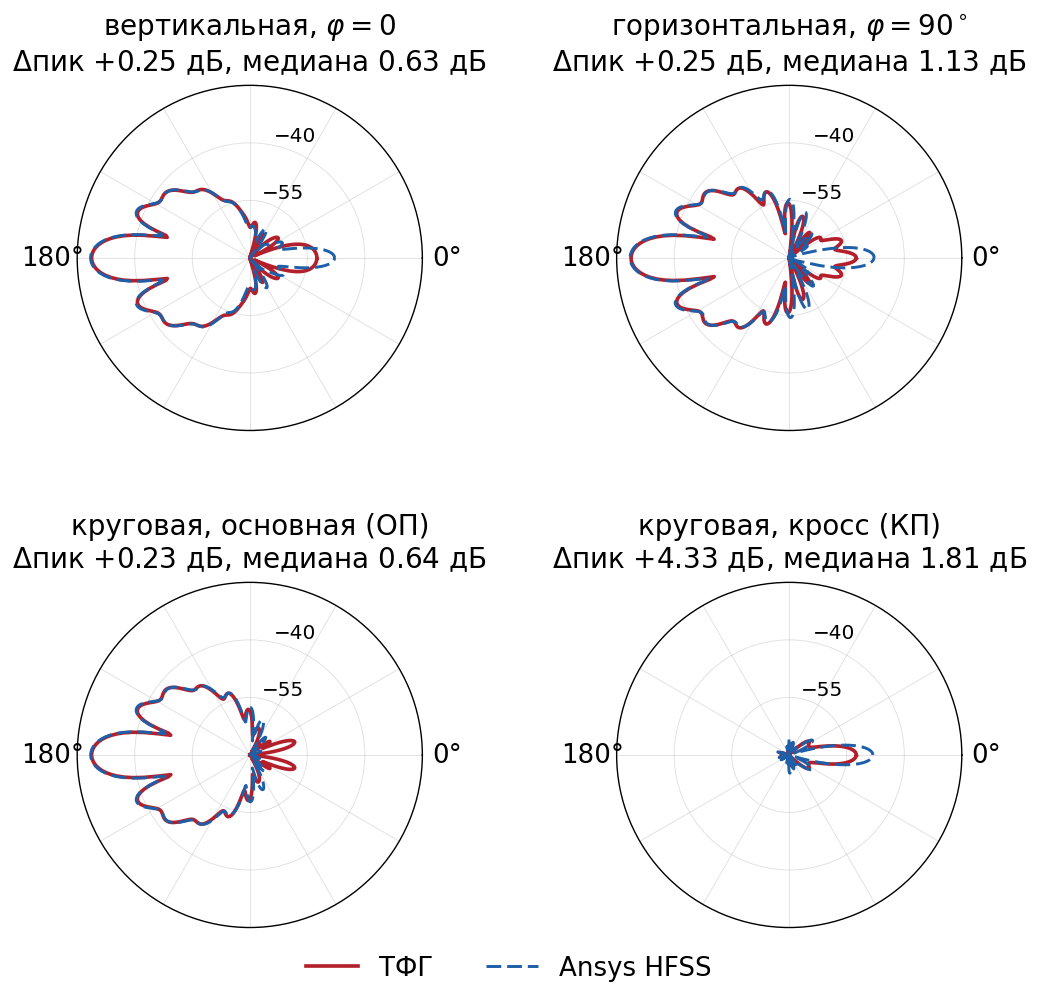
\includegraphics[width=0.98\textwidth]{pol_luneburg_k15_diffraction}
  \caption{Линза Люнеберга (пять слоёв), $k_0a = 15$: ненормированные диаграммы
  рассеяния метода ТФГ и полноволнового эталона}
  \label{fig:pol-lun}
\end{figure}

\FloatBarrier

\subsubsection{Ближняя зона}
\label{sec:res-near}

Помимо дальней зоны сопоставлено распределение поля в ближней зоне --- в плоскости
$xz$ на квадратной сетке $141\times141$, охватывающей тело и область до
$2\lambda_0$ вокруг него. Расчёт методом ТФГ ведётся точным радиальным рядом с
функциями $\hn(k_0r)$ \eqref{eq:near-Eth}--\eqref{eq:near-Er}, то есть
аналитическим продолжением того же ряда, чья асимптотика даёт диаграмму дальней
зоны; нормировка наследуется из дальней зоны аналитически.

Сопоставляется амплитуда рассеянного поля $|\vec E^{\,s}|$. Со стороны
полноволнового расчёта она собирается из комплексных компонент как
$|\vec E^{\,s}| = (|E_x|^2 + |E_y|^2 + |E_z|^2)^{1/2}$; выгрузка мгновенного
значения поля для этого непригодна, так как отличается от амплитуды множителем
$|\cos(k_0r+\psi)|$. Результаты приведены в таблице~\ref{tab:near}.

\begin{table}[ht]
  \centering
  \small
  \caption{Сверка ближней зоны по комплексным компонентам поля. Медианы взяты по
  узлам вне тела при уровне выше $1\,\%$ от максимума}
  \label{tab:near}
  \renewcommand{\arraystretch}{1.2}
  \begin{tabular}{@{}lcccc@{}}
    \toprule
    Тело & $k_0a$ & Медиана, дБ & Медиана отношения & $\Delta$ максимума, дБ \\
    \midrule
    \multirow{3}{*}{Проводящая сфера}
      & $0{,}5$ & $0{,}24$ & $0{,}973$ & $-0{,}02$ \\
      & $2$     & $0{,}19$ & $0{,}988$ & $-0{,}12$ \\
      & $15$    & $0{,}33$ & $0{,}989$ & $+0{,}18$ \\
    \midrule
    \multirow{3}{*}{Сфера с укрытием}
      & $0{,}5$ & $0{,}21$ & $0{,}976$ & $-0{,}15$ \\
      & $2$     & $0{,}21$ & $0{,}985$ & $-0{,}19$ \\
      & $15$    & $0{,}41$ & $1{,}013$ & $+0{,}22$ \\
    \midrule
    Линза Люнеберга & $15$ & $0{,}54$ & $0{,}985$ & $+0{,}03$ \\
    \midrule
    \multicolumn{2}{@{}l}{\textbf{Медиана по семи}} &
      $\mathbf{0{,}24}$ & $\mathbf{0{,}985}$ & $\mathbf{0{,}15}$ \\
    \bottomrule
  \end{tabular}
\end{table}

Карты приведены на рис.~\ref{fig:near}. Совпадает и интерференционная структура вне
тела, и уровень. Область внутри тела у метода ТФГ маскирована: ряд построен по
исходящим сферическим функциям $\hn(k_0r)$, расходящимся при $r\to0$, и вне области
своей сходимости смысла не имеет. У линзы Люнеберга полноволновой расчёт показывает
в этой области коллимацию волны слоями --- эффект, для описания которого требуются
амплитуды гармоник в слоях.

\begin{figure}[ht]
  \centering
  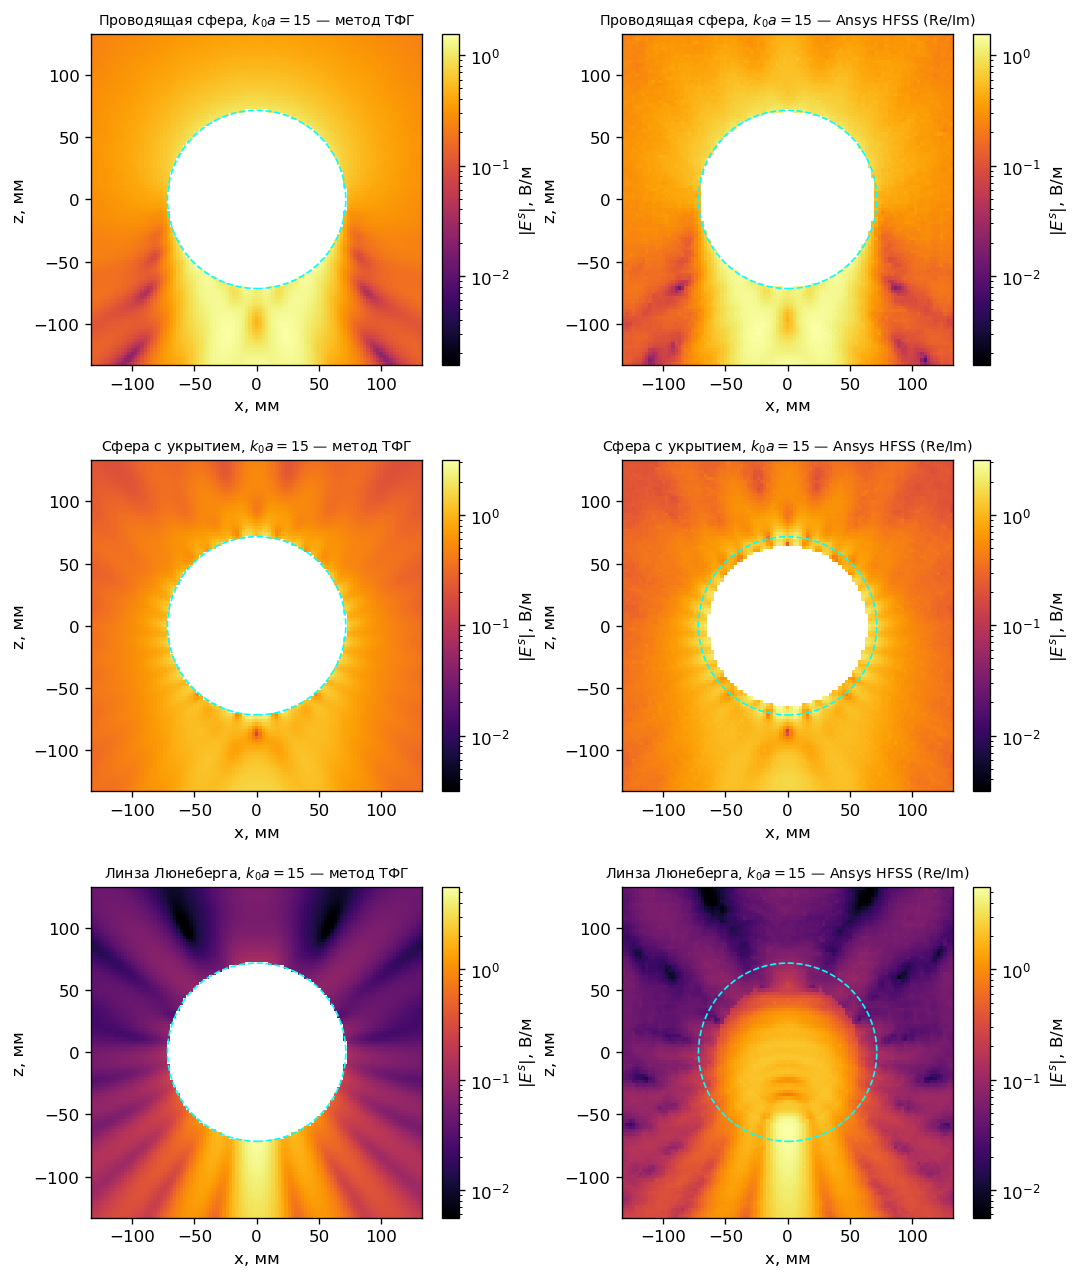
\includegraphics[width=0.99\textwidth]{near_cmp_vec}
  \caption{Ближняя зона при $k_0a = 15$, плоскость $xz$: модуль рассеянного поля
  $|\vec E^{\,s}|$ по методу ТФГ (слева) и полноволновому расчёту по комплексным
  компонентам (справа). Общая шкала и логарифмический диапазон 60~дБ внутри каждой
  пары; штриховой окружностью показана внешняя граница тела}
  \label{fig:near}
\end{figure}

\FloatBarrier

\subsubsection{Вывод по дифракционной задаче}
\label{sec:res-sum}

\begin{table}[ht]
  \centering
  \small
  \caption{Сверка ненормированных диаграмм с полноволновым эталоном, задача
  дифракции. Для каждой поляризации указаны расхождение максимумов $\Delta$ и
  медиана поточечного расхождения по лепесткам выше $1\,\%$ от максимума, дБ}
  \label{tab:verify-diff}
  \renewcommand{\arraystretch}{1.2}
  \begin{tabular}{@{}lcccccccc@{}}
    \toprule
    \multirow{2}{*}{Тело} & \multirow{2}{*}{$k_0a$} &
    \multicolumn{2}{c}{Вертикальная} & \multicolumn{2}{c}{Горизонтальная} &
    \multicolumn{2}{c}{Круговая, ОП} & \multicolumn{1}{c}{Круговая, КП} \\
    \cmidrule(lr){3-4}\cmidrule(lr){5-6}\cmidrule(lr){7-8}\cmidrule(lr){9-9}
    & & $\Delta$ & медиана & $\Delta$ & медиана & $\Delta$ & медиана & $\Delta$ / медиана \\
    \midrule
    \multirow{3}{*}{Проводящая сфера}
      & $0{,}5$ & $-0{,}29$ & $0{,}31$ & $+0{,}29$ & $0{,}39$ & $+0{,}43$ & $1{,}00$ & $-0{,}20$ / $0{,}29$ \\
      & $2$     & $+0{,}02$ & $0{,}10$ & $+0{,}04$ & $0{,}47$ & $-0{,}10$ & $0{,}45$ & $+0{,}43$ / $0{,}31$ \\
      & $15$    & $+0{,}23$ & $0{,}49$ & $+0{,}23$ & $0{,}50$ & $+0{,}18$ & $0{,}41$ & $+0{,}04$ / $0{,}39$ \\
    \midrule
    \multirow{3}{*}{Сфера с укрытием}
      & $0{,}5$ & $-0{,}36$ & $0{,}25$ & $-0{,}05$ & $0{,}21$ & $-0{,}26$ & $0{,}40$ & $-0{,}35$ / $0{,}16$ \\
      & $2$     & $+0{,}05$ & $0{,}14$ & $+0{,}06$ & $0{,}31$ & $-0{,}03$ & $0{,}29$ & $+0{,}23$ / $0{,}21$ \\
      & $15$    & $+0{,}26$ & $0{,}45$ & $+0{,}26$ & $0{,}59$ & $+0{,}23$ & $0{,}81$ & $+0{,}47$ / $0{,}43$ \\
    \midrule
    Линза Люнеберга
      & $15$    & $+0{,}25$ & $0{,}63$ & $+0{,}25$ & $1{,}13$ & $+0{,}23$ & $0{,}64$ & $+4{,}33$ / $1{,}81$ \\
    \midrule
    \multicolumn{2}{@{}l}{\textbf{Медиана по семи}} &
      $\mathbf{0{,}25}$ & $\mathbf{0{,}31}$ & $\mathbf{0{,}23}$ & $\mathbf{0{,}47}$ &
      $\mathbf{0{,}23}$ & $\mathbf{0{,}45}$ & $\mathbf{0{,}35}$ / $\mathbf{0{,}31}$ \\
    \bottomrule
  \end{tabular}
\end{table}

По всем 28 диаграммам дифракционной задачи медиана поточечного расхождения
составляет $0{,}40$~дБ при максимуме $1{,}81$~дБ, медиана расхождения максимумов ---
$0{,}23$~дБ. Все величины абсолютные: приведение кривых к максимуму не
применялось.

\clearpage
\section{Постановка антенной задачи}
\label{sec:antenna}

Во второй (антенной) задаче источник --- элементарный излучатель, моделирующий
рупорный облучатель, --- расположен непосредственно на внешней поверхности
структуры ($r = a$), и рассчитывается создаваемое им поле излучения
(рис.~\ref{fig:geom-ant}). Обе задачи различаются только видом возбуждения в
числителе коэффициентов рассеяния и решаются единым алгоритмом.

Тело для этой задачи выбрано единственное --- линза Люнеберга. Причина в том, что
антенный режим содержателен лишь для тела, прозрачного и фокусирующего: по
\eqref{eq:Emax} максимум поля лежит в направлении $\theta = \pi$, антиподальном
облучателю, то есть излучение проходит \emph{сквозь} тело. Для проводящей сферы и
сферы с укрытием это невозможно. Однородная шар-линза $\varepsilon = 4$ прозрачна,
но усиления не даёт ($0{,}709$~В/м против $0{,}753$~В/м у свободного облучателя)
вследствие сферической аберрации; линза Люнеберга апланатична по построению и
потому принята в качестве расчётного тела.

\begin{figure}[ht]
  \centering
  \begin{tikzpicture}[scale=1.05,>=latex]
    \fill[gray!10] (0,0) circle (1.55);
    \draw[thick] (0,0) circle (1.55);
    \draw[dashed,gray!70] (0,0) circle (1.10);
    \draw[dashed,gray!70] (0,0) circle (0.62);
    \node[font=\tiny] at (0,0.25) {$\varepsilon_1',\mu_1'$};
    \draw[->] (0,0) -- (0,2.45) node[right,font=\tiny]{$z$};
    \draw[->] (0,0) -- (2.15,0) node[below,font=\tiny]{$x$};
    \draw[dashed,orange!85!black,thick] plot[domain=0:360,samples=90,smooth cycle,
      variable=\t] ({0.78*(1+cos(\t))/2*sin(\t)},{1.55-0.78*(1+cos(\t))/2*cos(\t)});
    \draw[->,very thick,blue!70!black] (-0.32,1.55) -- (0.32,1.55);
    \node[blue!70!black,font=\tiny] at (0.95,1.62) {$I^{e}\!\parallel\!\ao$};
    \filldraw[fill=white,draw=green!45!black,very thick] (0,1.55) circle (0.10);
    \draw[green!45!black,very thick] (-0.07,1.48)--(0.07,1.62);
    \draw[green!45!black,very thick] (-0.07,1.62)--(0.07,1.48);
    \node[green!45!black,font=\tiny] at (-1.00,1.86) {$\dfrac{I^{m}}{Z_0}\!\parallel\!\af$};
    \node[orange!85!black,font=\tiny] at (1.42,0.82) {$\dfrac{1+\cos\theta}{2}$};
    \draw[->,thick,red!70!black] (0,0) -- (200:2.75)
      node[below left,font=\tiny,align=center]{$\vec E(r)$};
    \node[font=\tiny,gray!60!black] at (0,-1.95) {$\theta=180^\circ$ --- максимум излучения};
    \node[font=\tiny,gray!60!black] at (0,2.62) {$r=a$: источник на поверхности};
  \end{tikzpicture}
  \caption{Геометрия антенной задачи: элемент Гюйгенса на внешней поверхности
  структуры, ориентированный максимумом кардиоиды внутрь тела; максимум
  излучения --- в антиподальном направлении $\theta = 180^\circ$}
  \label{fig:geom-ant}
\end{figure}

\subsection{Теория: ненормированные значения напряжённости поля}
\label{sec:theory-ant}

Базовый аппарат тот же, что и в разделе~\ref{sec:theory-diff}; отличие режимов
сводится к числителю коэффициентов рассеяния. Облучателем служит элемент Гюйгенса
с амплитудой \eqref{eq:E0-huy} и собственной кардиоидной диаграммой
$(1+\cos\theta)/2$: источник однонаправлен и имеет нуль при $\theta = \pi$. Ниже
приведено только добавленное --- амплитудный пакет антенной задачи и
соотношение взаимности, по которому ведётся расчёт.

\paragraph{Коэффициенты рассеяния антенного режима.}
При источнике на поверхности падающая волна в постановке отсутствует, и след
падающей волны в числителе \eqref{eq:Mn} заменяется на единичное возбуждение
поверхности~\cite[ф-ла~13.4]{panchenko2013}:
%
\begin{align}
  \label{eq:MnNn-ant}
  M_n' &= \frac{j\Zl_n(a) - j}{j\Zb_n(a)\,\hn(k_0a)}, &
  N_n' &= \frac{j\Yl_n(a) - j}{j\Yb_n(a)\,\hn(k_0a)}.
\end{align}
%
Знаменатель и вся импедансная рекурсия остаются прежними --- отличие
режимов сводится к одной строке алгоритма.

\paragraph{Ненормированная напряжённость поля.}
Поле записывается с коэффициентами \eqref{eq:MnNn-ant}, фазовым весом
$e^{\,j\frac{\pi}{2}n}$ и дополнительным множителем
$1/(k_0a)$~\cite[ф-ла~13.3]{panchenko2013}:
%
\begin{multline}
  \label{eq:pack-ant}
  \vec E(\vec r) = E_0\,\frac{e^{-jk_0r}}{(k_0r)(k_0a)}
  \sum_{n=1}^{\infty}\frac{2n+1}{n(n+1)}\,e^{\,j\frac{\pi}{2}n}
  \Bigl\langle\bigl[\cos\varphi\,\tau_n(\theta)\,\ao - \sin\varphi\,\pi_n(\theta)\,\af\bigr]M_n'\\
  -\bigl[\cos\varphi\,\pi_n(\theta)\,\ao - \sin\varphi\,\tau_n(\theta)\,\af\bigr]N_n'\Bigr\rangle.
\end{multline}
%
Максимум напряжённости достигается в направлении $\theta = \pi$, $\varphi = 0$;
используя $\tau_n(\pi) = (-1)^n\frac{n(n+1)}{2}$,
$\pi_n(\pi) = (-1)^{n+1}\frac{n(n+1)}{2}$, получаем из
\eqref{eq:pack-ant}~\cite[ф-ла~13.5]{panchenko2013}
%
\begin{equation}
  \label{eq:Emax}
  E_\theta(r) = E_{\max} = E_0\cdot\frac{e^{-jk_0r}}{2(k_0r)(k_0a)}
  \sum_{n=1}^{\infty}(2n+1)\,e^{\,j\frac{\pi}{2}n}(-1)^n\bigl[M_n' + N_n'\bigr].
\end{equation}
%
Множитель $2$ в знаменателе возникает именно из угловых функций, что служит
внутренним контролем согласованности \eqref{eq:pack-ant} и \eqref{eq:Emax}.
Нормированная диаграмма направленности в главных
плоскостях~\cite[ф-ла~13.6]{panchenko2013}
%
\begin{equation}
  \label{eq:Fpat}
  F(\theta,0) = \frac{2\sum\limits_{n=1}^{\infty}\dfrac{2n+1}{n(n+1)}
    e^{\,j\frac{\pi}{2}n}\bigl[\tau_n(\theta)M_n' - \pi_n(\theta)N_n'\bigr]}
    {\sum\limits_{n=1}^{\infty}(2n+1)\,e^{\,j\frac{\pi}{2}n}(-1)^n\bigl[M_n' + N_n'\bigr]}
\end{equation}
%
получается делением \eqref{eq:pack-ant} на \eqref{eq:Emax}: именно здесь амплитудный
множитель сокращается, и именно его восстановление составляет предмет настоящей
работы.

\paragraph{Диаграмма направленности линзовой антенны.}
Запись \eqref{eq:pack-ant} отвечает единичному возбуждению поверхности: числитель
\eqref{eq:MnNn-ant} задаёт всем гармоникам равную амплитуду на границе, тогда как
физический облучатель определяет модальный спектр своим полем на радиусе
$r_d$~\cite{moroz2005,li1994,chew1976}. Амплитуда исходящей волны для источника вне
слоистой сферы имеет вид
%
\begin{equation}
  \label{eq:moroz-ref}
  D_{\gamma n} = a^{d}_{\gamma n}
  + \underbrace{\frac{T_{21;\gamma n}}{T_{11;\gamma n}}}_{{}=\;M_n,\;N_n}
  \tilde a^{d}_{\gamma n},
\end{equation}
%
где $\tilde a^{d}_{\gamma n}$ --- проекция тока источника на векторный мультиполь
при $r = r_d$, а отношение $T_{21;\gamma n}/T_{11;\gamma n}$ есть коэффициент
импедансной рекурсии \eqref{eq:Mn}~\cite[ф-лы~32--34]{moroz2005}.

Эквивалентная и более короткая форма записи получается из симметрии тензора Грина
$\overline{\overline{\Gamma}}(\mathbf r,\mathbf r')$ как билинейного функционала
двух точек. Для облучателя в виде элемента
Гюйгенса с электрическим током вдоль $\hat p_e$ и магнитным вдоль
$\hat p_m = \hat n\times\hat p_e$, расположенного в точке $\mathbf r_d$:
%
\begin{equation}
  \label{eq:recip}
  \boxed{\;
  rE(\hat u) = \frac{I^e k_0 l Z_0}{4\pi}\,
  \Bigl|\,\hat p_e\!\cdot\!\vec E^{\,\text{полн}}(\mathbf r_d)
  + Z_0\,\hat p_m\!\cdot\!\vec H^{\,\text{полн}}(\mathbf r_d)\Bigr|
  \quad[\text{В}],\;}
\end{equation}
%
где $\vec E^{\,\text{полн}}$, $\vec H^{\,\text{полн}}$ --- полные поля в точке
облучателя при \emph{единичной} плоской волне, приходящей с направления
наблюдения $\hat u$. Поскольку слоистая сфера симметрична относительно центра,
направления $\hat u$ отвечают положениям точки $\mathbf r_d$ на сфере радиуса
$r_d$ при неподвижной падающей волне, то есть тому же дифракционному расчёту.

Множитель в \eqref{eq:recip} следует из предельного перехода к свободному
пространству: при отсутствии тела величина в модуле равна $2(1+\cos\Theta)/2$, то
есть удвоенной кардиоиде элемента Гюйгенса, откуда
$E_0^{(\text{Гюйг})}/2 = I^ek_0lZ_0/(4\pi r)$. Тот же переход определяет знак
магнитного слагаемого: он отвечает ориентации кардиоиды максимумом внутрь тела.

Магнитное поле, входящее в \eqref{eq:recip}, описывается вторым тензором Грина того
же аппарата --- $\overline{\overline{G}}_{21}$, характеристические части которого
отличаются от $\overline{\overline{G}}_{11}$ перестановкой функции и её
производной~\cite{denisov2016tensors}:
%
\begin{equation}
  \label{eq:g21}
  \begin{aligned}
    g_{11} &= \frac{\partial\overleftarrow I/\partial(k_0r)}{j\Zb(a)\,\hn(k_0a)}, &
    f_{11} &= \frac{j\overleftarrow V}{j\Yb(a)\,\hn(k_0a)}
    &&\text{(электрическое поле)},\\
    g_{21} &= \frac{\overleftarrow I}{j\Zb(a)\,\hn(k_0a)}, &
    f_{21} &= \frac{j\,\partial\overleftarrow V/\partial(k_0r)}{j\Yb(a)\,\hn(k_0a)}
    &&\text{(магнитное поле)}.
  \end{aligned}
\end{equation}
%
В сборке ряда это отвечает замене $M_n\leftrightarrow N_n$ и
$\cos\varphi\leftrightarrow\sin\varphi$ при общем множителе $1/Z_0$: в
электрическом поле коэффициент от импеданса стоит при производной
$[\rho\hn]'/\rho$, а от адмиттанса --- при функции $\hn$, в магнитном --- наоборот.

\subsection{Реализация в библиотеке GreenTensor}
\label{sec:impl-ant}

Переключение режима по \eqref{eq:MnNn-ant} реализовано одной ветвью в
\texttt{calculate\_scattering\_coefficients} (листинг~\ref{lst:coeffs}): при
\texttt{problem == "antenna"} числитель принимает вид \texttt{Zo - 1j}, что и есть
$j\Zl_n(a) - j$; знаменатель записан в эквивалентной форме
$j\Zl_n(a)\hn(k_0a) - \hn{}'(k_0a)$. Импедансная рекурсия, угловые функции и
сборка компонент --- общие для обоих режимов.

\begin{lstlisting}[style=py,caption={\texttt{green\_tensor/01\_sphere.py::calculate\_scattering\_coefficients}
--- переключение режима возбуждения},label={lst:coeffs}]
if self.problem == "antenna":
    self.Mn[i] = (Zo - 1j) / (Zo * self.mH[i] - self.mHpr[i])
    self.Nn[i] = (Yo - 1j) / (Yo * self.mH[i] - self.mHpr[i])
else:
    self.Mn[i] = (Zo * self.mJ[i] - self.mJpr[i]) / (Zo * self.mH[i] - self.mHpr[i])
    self.Nn[i] = (Yo * self.mJ[i] - self.mJpr[i]) / (Yo * self.mH[i] - self.mHpr[i])
self.Mn[i] = self.Mn[i].real - self.Mn[i].imag * 1j
self.Nn[i] = self.Nn[i].real - self.Nn[i].imag * 1j
\end{lstlisting}

Как показано в разделе~\ref{sec:results-ant}, этот путь абсолютного уровня не даёт.
Расчёт диаграммы направленности ведётся по соотношению взаимности
\eqref{eq:recip}, то есть на дифракционном решении. Для этого в модуль
\texttt{nearfield.py} добавлены две функции.

\paragraph{Магнитное поле.}
\texttt{magnetic\_field\_sphere} --- дуальная сборка того же ряда, что и
\eqref{eq:near-Eth}--\eqref{eq:near-Er}: замена $a_n\leftrightarrow b_n$,
$\cos\varphi\leftrightarrow\sin\varphi$ и общий множитель $1/Z_0$. Форма проверена
независимо: совпадает с $\nabla\times\vec E/(jk_0Z_0)$, вычисленным численным
дифференцированием аналитического поля, до $4\cdot10^{-7}$ в обоих направлениях
падения, для рассеянного и полного поля, в случайных точках вне главных плоскостей.

\begin{lstlisting}[style=py,caption={\texttt{nearfield.py::\_series} ---
дуальная сборка магнитного поля},label={lst:mag}]
if want == "E":
    c1, c2 = an[:, None], bn[:, None]
    f_th, f_ph, scale = np.cos(phi), -np.sin(phi), 1.0
else:                       # H: a<->b, cos<->sin, общий множитель 1/Z0
    c1, c2 = bn[:, None], an[:, None]
    f_th, f_ph, scale = np.sin(phi), np.cos(phi), 1.0 / z0

Fth = A * scale * np.sum(w * (1j * c1 * taun * D - c2 * pin * h), axis=0) * f_th
Fph = A * scale * np.sum(w * (1j * c1 * pin * D - c2 * taun * h), axis=0) * f_ph
\end{lstlisting}

Диаграмма направленности \eqref{eq:recip} собирается функцией
\texttt{antenna\_pattern\_sphere} в двух главных плоскостях.

\subsection{Верификационная модель в Ansys HFSS}
\label{sec:model-ant}

\paragraph{Рассматриваемый случай.}
Тело --- та же пятислойная линза Люнеберга, что и в дифракционной задаче
(таблица~\ref{tab:geom}), $k_0a = 15$, $a = 71{,}5702$~мм, $N_{\max} = 27$.
Диаметр линзы составляет $D = 2a = 4{,}775\lambda_0$.

\paragraph{Параметры источника.}
Облучатель реализован как элемент Гюйгенса --- пара скрещённых тангенциальных
токов на поверхности линзы --- с током $I^{e} = 1$~А и длиной
$l = \lambda_0/50 = 0{,}5996$~мм, ориентированный максимумом кардиоиды
\emph{внутрь} тела. Приёмка источника выполнена отдельным прогоном в свободном
пространстве: глубина нуля кардиоиды $-310$~дБ, расхождение формы с
$(1+\cos\theta)/2$ по медиане $0{,}43$~дБ, абсолютный уровень
$0{,}753461$~В/м на расстоянии $r = 10$~м. Расчётное значение по \eqref{eq:E0-huy}
при тех же параметрах составляет $I^{e}k_0lZ_0/(2\pi r) = Z_0/500 = 0{,}753461$~В/м:
источники совпадают с относительной погрешностью $1{,}3\cdot10^{-7}$.

\paragraph{Постановка эталонного расчёта.}
Постановка совпадает с дифракционной (раздел~\ref{sec:model-diff}) с заменой
возбуждения: вместо плоской волны --- элемент Гюйгенса на поверхности. Сетка
существенно плотнее из-за локализованного источника: $728\,033$ тетраэдра против
$41\,126$ в дифракционном прогоне того же тела. Модель приведена на
рис.~\ref{fig:model-ant}.

\begin{figure}[ht]
  \centering
  \begin{subfigure}[b]{0.47\textwidth}
    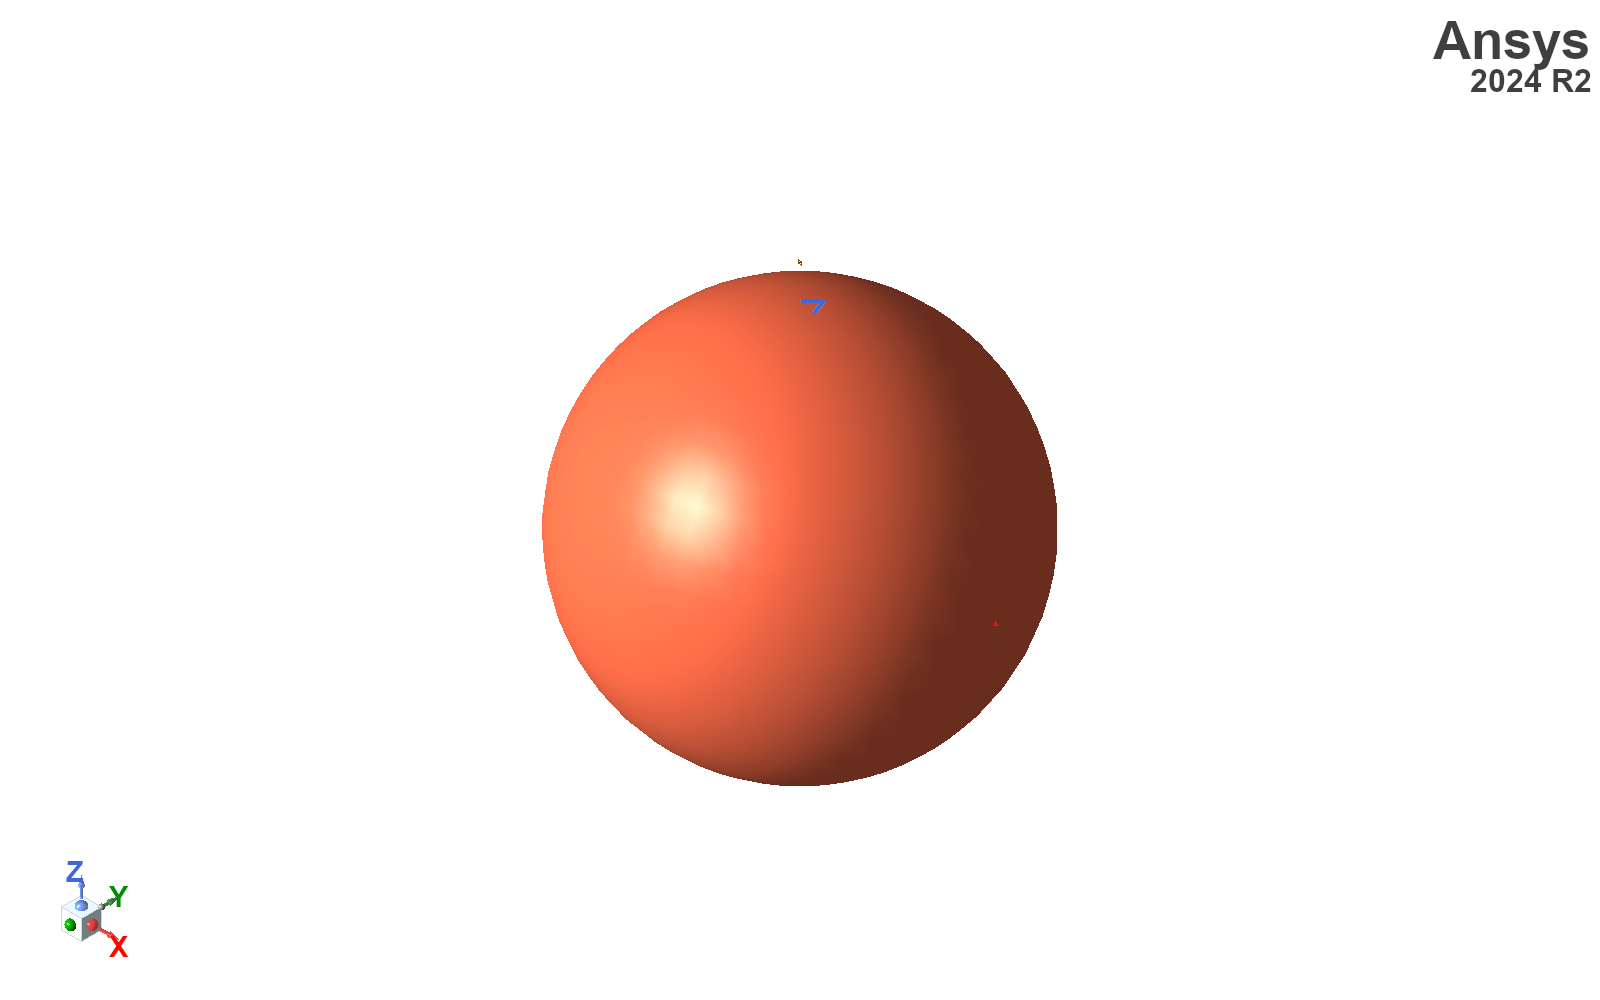
\includegraphics[width=\textwidth]{luneburg_k15_lens_src_iso}
    \caption{облучатель на поверхности линзы}
  \end{subfigure}\hfill
  \begin{subfigure}[b]{0.47\textwidth}
    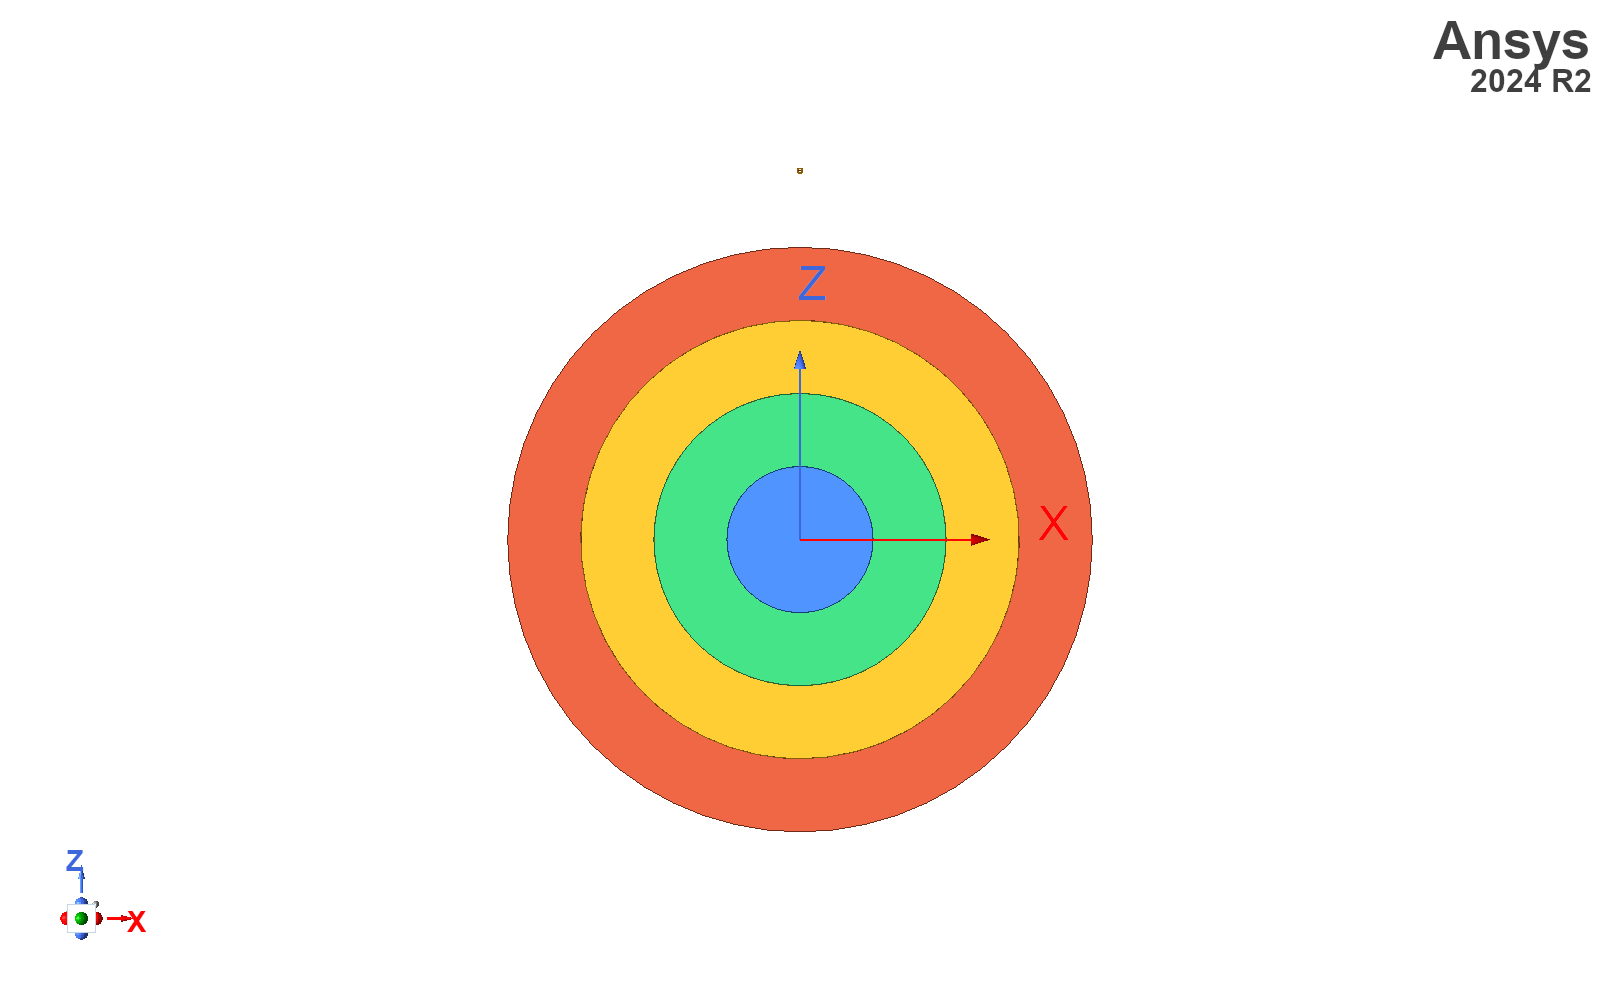
\includegraphics[width=\textwidth]{luneburg_k15_lens_cutaway_front}
    \caption{разрез: слоистая структура}
  \end{subfigure}
  \caption{Эталонная модель антенной задачи в Ansys HFSS: пятислойная линза
  Люнеберга с элементом Гюйгенса на внешней поверхности}
  \label{fig:model-ant}
\end{figure}

\subsection{Результаты верификации}
\label{sec:results-ant}

Набор диаграмм построен по тем же правилам, что и в дифракционной задаче
(раздел~\ref{sec:results-diff}): слева вертикальная поляризация (E-плоскость,
$\varphi = 0$), справа горизонтальная (H-плоскость, $\varphi = 90^\circ$), на каждой
диаграмме одна пара кривых, ориентация одинакова ($\theta = 0$ вверху, отсчёт по
часовой стрелке), радиальная шкала --- $20\lg|E|$ при $|E|$ в В/м, единая для обеих
диаграмм, динамический диапазон 45~дБ. Медиана расхождения вычислена по лепесткам
выше $1\,\%$ от максимума.

\begin{figure}[ht]
  \centering
  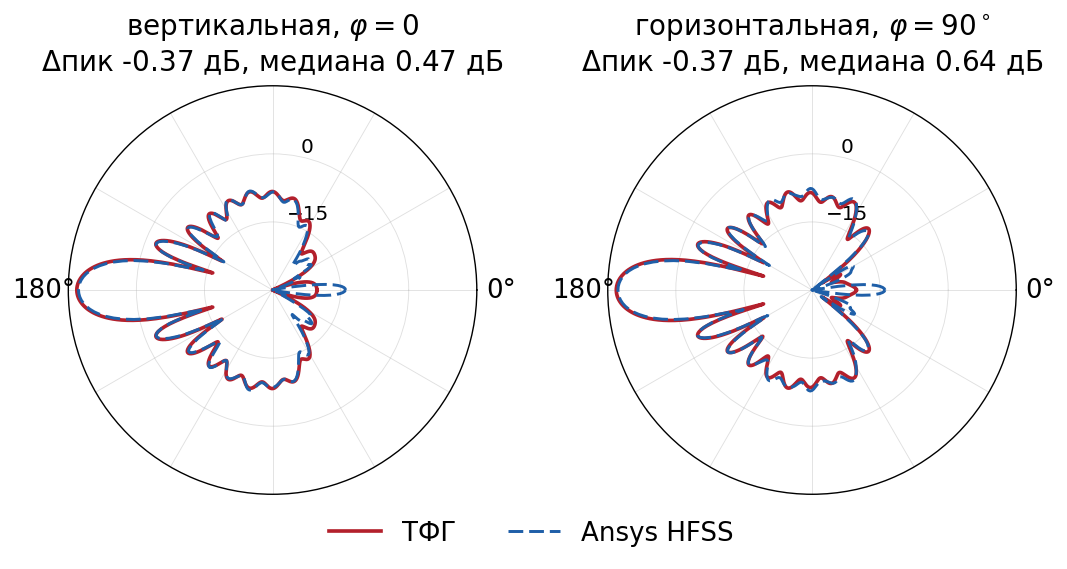
\includegraphics[width=0.98\textwidth]{pol_luneburg_k15_antenna}
  \caption{Линза Люнеберга, $k_0a = 15$, антенная задача: ненормированные диаграммы
  направленности метода ТФГ и полноволнового эталона}
  \label{fig:pol-lun-ant}
\end{figure}

\paragraph{Вывод.}
Диаграмма имеет вид, характерный для линзовой антенны: узкий главный лепесток в
направлении $\theta = 180^\circ$, антиподальном облучателю, то есть излучение
проходит сквозь тело и коллимируется слоями. Ширина главного лепестка по уровню
$-3$~дБ составляет $13{,}8^\circ$ против $13{,}6^\circ$ у полноволнового расчёта;
первый боковой лепесток --- $-15{,}5$ против $-15{,}2$~дБ. Обе величины
согласуются и лежат \emph{шире} однородно возбуждённой апертуры того же диаметра
($12{,}2^\circ$ при боковых $-17{,}6$~дБ), что отвечает спаду возбуждения к краям
от кардиоиды облучателя --- физически ожидаемому поведению.

Абсолютный уровень: максимум $4{,}531$~В/м против $4{,}342$~В/м у эталона,
расхождение $-0{,}37$~дБ. Относительно того же облучателя без тела
($0{,}753461$~В/м) это даёт усиление линзы $+15{,}58$~дБ по методу ТФГ и
$+15{,}21$~дБ по полноволновому расчёту. С учётом собственной направленности
кардиоиды ($\approx4{,}8$~дБи) итог $\approx20$~дБи при апертурном пределе
$(\pi D/\lambda_0)^2 = 23{,}5$~дБи для $D = 4{,}775\lambda_0$ --- предел не
нарушен.

Медиана поточечного расхождения по всей диаграмме составляет $0{,}47$~дБ в
E-плоскости и $0{,}64$~дБ в H-плоскости --- тот же уровень, что и в дифракционной
задаче (таблица~\ref{tab:verify-diff}), где медиана по 28 диаграммам равна
$0{,}40$~дБ. Распределение остатка по угловым секторам от максимума таково:
$0{,}51$~дБ в пределах $\pm20^\circ$ (главный лепесток), $0{,}34$~дБ в
$20\ldots60^\circ$, $0{,}17$~дБ в $60\ldots120^\circ$ и $2{,}17$; $4{,}46$~дБ в
секторах $120\ldots170^\circ$ и $170\ldots180^\circ$. Последние два отвечают
области вокруг направления $\theta\approx0$, отвечающего нулю кардиоиды
облучателя: медианный уровень поля там $-32$ и $-34$~дБ от максимума, и результат
сеточного метода чувствителен к дискретизации. Наибольшее единичное расхождение
($11{,}6$~дБ) приходится на $\theta = 16^\circ$ при уровне $-37{,}3$~дБ, то есть на
глубокий минимум.

\begin{table}[ht]
  \centering
  \small
  \caption{Сверка ненормированных диаграмм направленности с полноволновым
  эталоном, антенная задача}
  \label{tab:verify-ant}
  \renewcommand{\arraystretch}{1.2}
  \begin{tabular}{@{}lcccc@{}}
    \toprule
    \multirow{2}{*}{Тело} & \multirow{2}{*}{$k_0a$} &
    \multicolumn{1}{c}{Вертикальная} & \multicolumn{1}{c}{Горизонтальная} &
    \multirow{2}{*}{Кросс-поляризация} \\
    \cmidrule(lr){3-3}\cmidrule(lr){4-4}
    & & $\Delta$ / медиана & $\Delta$ / медиана & \\
    \midrule
    Линза Люнеберга & $15$ & $-0{,}37$ / $0{,}47$ & $-0{,}37$ / $0{,}64$ &
      ТФГ $0$; FEM $1{,}4\cdot10^{-2}$~В/м \\
    \midrule
    \multicolumn{5}{@{}l}{\emph{Показатели главного лепестка:}} \\
    \multicolumn{2}{@{}l}{Ширина по $-3$~дБ} &
      \multicolumn{1}{c}{ТФГ $13{,}8^\circ$} &
      \multicolumn{1}{c}{FEM $13{,}6^\circ$} &
      однородная апертура $12{,}2^\circ$ \\
    \multicolumn{2}{@{}l}{Первый боковой} &
      \multicolumn{1}{c}{ТФГ $-15{,}5$~дБ} &
      \multicolumn{1}{c}{FEM $-15{,}2$~дБ} &
      однородная апертура $-17{,}6$~дБ \\
    \multicolumn{2}{@{}l}{Максимум $|E|$, В/м} &
      \multicolumn{1}{c}{ТФГ $4{,}531$} &
      \multicolumn{1}{c}{FEM $4{,}342$} &
      свободный облучатель $0{,}753$ \\
    \multicolumn{2}{@{}l}{Усиление линзы} &
      \multicolumn{1}{c}{ТФГ $+15{,}58$~дБ} &
      \multicolumn{1}{c}{FEM $+15{,}21$~дБ} &
      апертурный предел $23{,}5$~дБи \\
    \bottomrule
  \end{tabular}
\end{table}

\FloatBarrier

\section{Выводы}
\label{sec:conclusion}

\paragraph{Реализовано.}
Амплитудный множитель $E_0$, сокращающийся при переходе к нормированной диаграмме
\eqref{eq:Fpat} и потому опускаемый в теоретической записи, восстановлен в
библиотеке GreenTensor в замкнутой форме для обоих режимов возбуждения. Расчёт даёт
напряжённость поля в вольтах на метр: дифракционный режим --- по \eqref{eq:abs-lin}
и \eqref{eq:circR}--\eqref{eq:circL}, антенный --- по \eqref{eq:pack-ant} с
амплитудой источника \eqref{eq:E0} либо \eqref{eq:E0-huy}. Множитель $1/2$ круговой
поляризации выведен, а не подобран. Поле в ближней зоне вычисляется точным
радиальным рядом с функциями $\hn(k_0r)$ --- строгим аналитическим продолжением
того же ряда, чья асимптотика даёт диаграмму.

\paragraph{Верифицировано.}
\begin{itemize}
  \item \textbf{Дифракционная задача --- подтверждена полностью} на семи
        конфигурациях: проводящая сфера и сфера с диэлектрическим укрытием при
        $k_0a = 0{,}5$; $2$; $15$ и линза Люнеберга при $k_0a = 15$.
        По всем 28 диаграммам медиана поточечного расхождения $0{,}40$~дБ при
        максимуме $1{,}81$~дБ, медиана расхождения максимумов $0{,}23$~дБ
        (таблица~\ref{tab:verify-diff}). Согласие достигнуто по абсолютной величине,
        без приведения кривых к максимуму.
  \item \textbf{Круговая поляризация} подтверждена наравне с линейной: медианы по
        основной и кросс-поляризации $0{,}45$ и $0{,}31$~дБ. Соответствие рукости
        $E_{op}\leftrightarrow$~RHCP согласовано во всех семи конфигурациях, что
        служит независимым подтверждением выведенного множителя $1/2$.
  \item \textbf{Кросс-поляризация линейной задачи} даёт у метода тождественный нуль
        ($E_\varphi$), у полноволнового расчёта --- на $31\ldots52$~дБ ниже
        основной составляющей, то есть на уровне численного шума сетки.
  \item \textbf{Ближняя зона} --- медиана $0{,}24$~дБ по семи конфигурациям при
        медиане отношения $0{,}985$ (таблица~\ref{tab:near}). Прежнее расхождение
        около $3$~дБ опознано как формат выгрузки эталона (мгновенное поле вместо
        амплитуды) и снято переходом к комплексным компонентам, без изменения
        расчёта.
  \item \textbf{Физическая картина} воспроизводится согласованно обеими методиками:
        переход от рэлеевского рассеяния с преобладанием обратного направления
        ($-7{,}26$~дБ вперёд/назад при $k_0a = 0{,}5$) к квазиоптическому с
        концентрацией поля вперёд ($+24{,}02$~дБ при $k_0a = 15$), сужение главного
        лепестка укрытием, усиление обратного рассеяния слоем на $4{,}61$~дБ.
\end{itemize}

\paragraph{Антенная задача.}
Запись \eqref{eq:pack-ant} отвечает единичному возбуждению поверхности и потому
абсолютного уровня не задаёт: модальный спектр \eqref{eq:MnNn-ant} не связан с
полем реального облучателя. Модальные амплитуды источника, стоящие в
\eqref{eq:moroz-ref}, строятся на радиусе $r_d$~\cite{moroz2005,li1994,chew1976},
причём отношение $T_{21}/T_{11}$ совпадает с коэффициентом импедансной рекурсии
\eqref{eq:Mn}, то есть новых коэффициентов задача не требует.

Расчёт выполняется по эквивалентной форме \eqref{eq:recip}, следующей из симметрии
тензора Грина, --- целиком на дифракционном решении. Согласие с эталоном отвечает
уровню дифракционной ветви: расхождение максимумов $-0{,}37$~дБ при абсолютном
уровне $4{,}531$ против $4{,}342$~В/м, медиана по лепесткам $0{,}47$~дБ
(E-плоскость) и $0{,}64$~дБ (H-плоскость), ширина луча $13{,}8^\circ$ против
$13{,}6^\circ$, первый боковой $-15{,}5$ против $-15{,}2$~дБ
(таблица~\ref{tab:verify-ant}).

Магнитное поле, входящее в \eqref{eq:recip}, вычисляется по \eqref{eq:g21} ---
второму тензору Грина того же аппарата; в библиотеке ему отвечает функция
\texttt{magnetic\_field\_sphere}, диаграмме направленности ---
\texttt{antenna\_pattern\_sphere}.

\subsection{Вычислительные затраты}
\label{sec:cost}

\paragraph{Вычислительная платформа.}
Полноволновые расчёты выполнены на рабочей станции AMD Ryzen 9 7950X3D
(16 ядер / 32 потока), NVIDIA GeForce RTX 4080 Super, оперативная память
DDR5-8000. Расчёты методом ТФГ выполнены на Apple M2 Pro (12 ядер), 16~ГБ
оперативной памяти, в один поток. Платформы, таким образом, \emph{разные}, причём
менее производительная досталась методу ТФГ; приведённые ниже отношения по времени
следует понимать как оценку порядка, а не как измерение на одинаковом железе.
Отношения по памяти от платформы не зависят --- это объём, необходимый для
хранения решения.

\begin{table}[ht]
  \centering
  \small
  \caption{Вычислительные затраты. Нагрузка метода ТФГ в дифракционных строках ---
  три диаграммы на сетке $360$ узлов, карта ближней зоны $141\times141$ и карта
  дальней зоны $73\times60$; в антенной строке --- два среза диаграммы
  направленности по $1440$ углов. Память --- пиковая по \texttt{tracemalloc}}
  \label{tab:cost}
  \renewcommand{\arraystretch}{1.2}
  \begin{tabular}{@{}lccccccc@{}}
    \toprule
    \multirow{2}{*}{Тело} & \multirow{2}{*}{$k_0a$} &
    \multicolumn{3}{c}{Полноволновой метод (FEM)} &
    \multicolumn{2}{c}{Метод ТФГ} & \multirow{2}{*}{Выигрыш} \\
    \cmidrule(lr){3-5}\cmidrule(lr){6-7}
    & & тетраэдры & память & время & память & время & память / время \\
    \midrule
    \multicolumn{8}{@{}l}{\emph{Задача дифракции:}} \\
    \multirow{3}{*}{Проводящая сфера}
      & $0{,}5$ & 5\,564  & 393 МБ     & 141 с   & $24{,}9$ МБ & $2{,}1$ с & $\times16$ / $\times68$ \\
      & $2$     & 5\,839  & 392 МБ     & 130 с   & $19{,}3$ МБ & $2{,}5$ с & $\times20$ / $\times53$ \\
      & $15$    & 69\,638 & $4{,}1$ ГБ & 921 с   & $46{,}3$ МБ & $6{,}7$ с & $\times89$ / $\times138$ \\
    \midrule
    \multirow{3}{*}{Сфера с укрытием}
      & $0{,}5$ & 14\,359 & 614 МБ     & 139 с    & $13{,}4$ МБ & $1{,}5$ с & $\times46$ / $\times95$ \\
      & $2$     & 10\,689 & 773 МБ     & 130 с    & $19{,}3$ МБ & $2{,}5$ с & $\times40$ / $\times52$ \\
      & $15$    & 97\,017 & $6{,}6$ ГБ & 1\,025 с & $46{,}3$ МБ & $6{,}8$ с & $\times143$ / $\times151$ \\
    \midrule
    Линза Люнеберга
      & $15$    & 41\,126 & $3{,}9$ ГБ & 1\,380 с & $46{,}3$ МБ & $7{,}2$ с & $\times86$ / $\times192$ \\
    \midrule
    \multicolumn{8}{@{}l}{\emph{Антенная задача:}} \\
    Линза Люнеберга
      & $15$    & \textbf{728\,033} & \textbf{47 ГБ} & \textbf{3\,480 с} &
        $\mathbf{3{,}8}$ \textbf{МБ} & $\mathbf{4{,}8}$ \textbf{с} &
        --- / $\mathbf{\times731}$ \\
    \bottomrule
  \end{tabular}
\end{table}

Наибольшее различие затрат даёт антенная задача. Локализованный источник на
поверхности требует существенно более плотной сетки: $728$~тыс.\ тетраэдров против
$41$~тыс.\ в дифракционном прогоне того же тела, то есть в $17{,}7$ раза. Расход
памяти при этом составляет $47$~ГБ, а время решения --- $58$~минут. Расчёт по
\eqref{eq:recip} даёт оба среза диаграммы за $4{,}8$~секунды, то есть в $731$ раз
быстрее. Отношение по памяти для этой строки не приводится: нагрузки не
сопоставимы --- полноволновой расчёт строит решение во всём объёме, тогда как
\eqref{eq:recip} обращается к полю в единственной точке $\mathbf r_d$.

Отметим, что $47$~ГБ --- это не характеристика реализации, а объём, необходимый
для хранения решения на сетке такого размера. Он превышает типичный объём
оперативной памяти рабочей станции, и именно этим ограничивается измельчение сетки:
дальнейшее уточнение полноволнового результата требует уже не времени, а другого
класса машины. Для метода ТФГ такого ограничения нет --- число удерживаемых
гармоник $N_{\max}\sim k_0a$ растёт линейно, тогда как число тетраэдров сеточного
метода --- как $(k_0a)^3$.

В дифракционной задаче на том же теле различие меньше ($\times86$ по памяти при
$3{,}9$~ГБ), поскольку плоская волна не требует локального измельчения сетки у
источника.

\begin{thebibliography}{9}
\bibitem{denisov2016tensors}
  Денисов, Д.\,В., Скуматенко, И.\,О. Тензорные функции Грина для решения задач
  электромагнитной дифракции на многослойных сферических структурах.
\bibitem{panchenko2013}
  Панченко, Б.\,А. Рассеяние и поглощение электромагнитных волн неоднородными
  сферическими телами. --- М.: Радиотехника, 2013. --- 264~с.
\bibitem{PanchenkoLA}
  Панченко, Б.\,А., Соколов, В.\,Ф. Радиопрозрачные конструкции летательных
  аппаратов. --- М.: Машиностроение, 1983. --- 216~с.
\bibitem{aden1951}
  Aden, A.\,L., Kerker, M. Scattering of Electromagnetic Waves from Two Concentric
  Spheres~// Journal of Applied Physics. --- 1951. --- Vol.~22, no.~10. ---
  P.~1242--1246.
\bibitem{bohren1983}
  Bohren, C.\,F., Huffman, D.\,R. Absorption and Scattering of Light by Small
  Particles. --- New York: Wiley, 1983.
\bibitem{wiscombe1980}
  Wiscombe, W.\,J. Improved Mie scattering algorithms~// Applied Optics. --- 1980.
  --- Vol.~19, no.~9. --- P.~1505--1509.
\bibitem{moroz2005}
  Moroz, A. A recursive transfer-matrix solution for a dipole radiating inside and
  outside a stratified sphere~// Annals of Physics. --- 2005. --- Vol.~315, no.~2.
  --- P.~352--418. (Референсная программа доступна на
  \texttt{wave-scattering.com}.)
\bibitem{li1994}
  Li, L.-W., Kooi, P.-S., Leong, M.-S., Yeo, T.-S. Electromagnetic dyadic Green's
  function in spherically multilayered media~// IEEE Transactions on Microwave
  Theory and Techniques. --- 1994. --- Vol.~42, no.~12. --- P.~2302--2310.
\bibitem{chew1976}
  Chew, H., McNulty, P.\,J., Kerker, M. Model for Raman and fluorescent scattering
  by molecules embedded in small particles~// Physical Review A. --- 1976. ---
  Vol.~13, no.~1. --- P.~396--404.
\bibitem{gaponenko2021}
  Gaponenko, R., Moroz, A., Rasskazov, I.\,L., Ladutenko, K., Shcherbakov, A.,
  Belov, P. Harnessing superdirectivity in dielectric spherical multilayer
  antennas~// Physical Review B. --- 2021. --- Vol.~104. --- P.~195406.
\bibitem{harrington1960}
  Harrington, R.\,F. Effect of antenna size on gain, bandwidth, and efficiency~//
  Journal of Research of the National Bureau of Standards. --- 1960. ---
  Vol.~64D, no.~1. --- P.~1--12.
\bibitem{luneburg1944}
  Luneburg, R.\,K. Mathematical Theory of Optics. --- Providence: Brown University,
  1944. --- 400~p. (Линза с профилем $\varepsilon(r) = 2 - (r/a)^2$, \S\,29.)
\end{thebibliography}

\end{document}
